% Options for packages loaded elsewhere
\PassOptionsToPackage{unicode}{hyperref}
\PassOptionsToPackage{hyphens}{url}
\PassOptionsToPackage{dvipsnames,svgnames,x11names}{xcolor}
\PassOptionsToPackage{space}{xeCJK}
\documentclass[
  10pt,
  a4paper,
]{ctexart}
\usepackage{xcolor}
\usepackage[margin=0.8in]{geometry}
\usepackage{amsmath,amssymb}
\setcounter{secnumdepth}{-\maxdimen} % remove section numbering
\usepackage{iftex}
\ifPDFTeX
  \usepackage[T1]{fontenc}
  \usepackage[utf8]{inputenc}
  \usepackage{textcomp} % provide euro and other symbols
\else % if luatex or xetex
  \usepackage{unicode-math} % this also loads fontspec
  \defaultfontfeatures{Scale=MatchLowercase}
  \defaultfontfeatures[\rmfamily]{Ligatures=TeX,Scale=1}
\fi
\usepackage{lmodern}
\ifPDFTeX\else
  % xetex/luatex font selection
  \setmainfont[]{Times New Roman}
  \setmonofont[]{Consolas}
  \ifXeTeX
    \usepackage{xeCJK}
    \setCJKmainfont[]{Microsoft YaHei}
  \fi
  \ifLuaTeX
    \usepackage[]{luatexja-fontspec}
    \setmainjfont[]{Microsoft YaHei}
  \fi
\fi
% Use upquote if available, for straight quotes in verbatim environments
\IfFileExists{upquote.sty}{\usepackage{upquote}}{}
\IfFileExists{microtype.sty}{% use microtype if available
  \usepackage[]{microtype}
  \UseMicrotypeSet[protrusion]{basicmath} % disable protrusion for tt fonts
}{}
\makeatletter
\@ifundefined{KOMAClassName}{% if non-KOMA class
  \IfFileExists{parskip.sty}{%
    \usepackage{parskip}
  }{% else
    \setlength{\parindent}{0pt}
    \setlength{\parskip}{6pt plus 2pt minus 1pt}}
}{% if KOMA class
  \KOMAoptions{parskip=half}}
\makeatother
\usepackage{longtable,booktabs,array}
\newcounter{none} % for unnumbered tables
\usepackage{calc} % for calculating minipage widths
% Correct order of tables after \paragraph or \subparagraph
\usepackage{etoolbox}
\makeatletter
\patchcmd\longtable{\par}{\if@noskipsec\mbox{}\fi\par}{}{}
\makeatother
% Allow footnotes in longtable head/foot
\IfFileExists{footnotehyper.sty}{\usepackage{footnotehyper}}{\usepackage{footnote}}
\makesavenoteenv{longtable}
\usepackage{graphicx}
\makeatletter
\newsavebox\pandoc@box
\newcommand*\pandocbounded[1]{% scales image to fit in text height/width
  \sbox\pandoc@box{#1}%
  \Gscale@div\@tempa{\textheight}{\dimexpr\ht\pandoc@box+\dp\pandoc@box\relax}%
  \Gscale@div\@tempb{\linewidth}{\wd\pandoc@box}%
  \ifdim\@tempb\p@<\@tempa\p@\let\@tempa\@tempb\fi% select the smaller of both
  \ifdim\@tempa\p@<\p@\scalebox{\@tempa}{\usebox\pandoc@box}%
  \else\usebox{\pandoc@box}%
  \fi%
}
% Set default figure placement to htbp
\def\fps@figure{htbp}
\makeatother
\setlength{\emergencystretch}{3em} % prevent overfull lines
\providecommand{\tightlist}{%
  \setlength{\itemsep}{0pt}\setlength{\parskip}{0pt}}
\usepackage{bookmark}
\IfFileExists{xurl.sty}{\usepackage{xurl}}{} % add URL line breaks if available
\urlstyle{same}
\hypersetup{
  colorlinks=true,
  linkcolor={Maroon},
  filecolor={Maroon},
  citecolor={Blue},
  urlcolor={Blue},
  pdfcreator={LaTeX via pandoc}}

\author{}
\date{}

\begin{document}

\section{Geant4-Sentaurus 耦合仿真的 4H-SiC PIN C-14 β 探测器设计优化：i
区厚度与外延缺陷密度的权衡}\label{geant4-sentaurus-ux8026ux5408ux4effux771fux7684-4h-sic-pin-c-14-ux3b2-ux63a2ux6d4bux5668ux8bbeux8ba1ux4f18ux5316i-ux533aux539aux5ea6ux4e0eux5916ux5ef6ux7f3aux9677ux5bc6ux5ea6ux7684ux6743ux8861}

\subsection{摘要}\label{ux6458ux8981}

4H-SiC 具有宽禁带、低暗电流和高辐照耐受性，是室温 C-14 β
探测器的重要候选材料。本文建立 Geant4-Sentaurus 耦合仿真框架，将 C-14
连续 β 谱及若干单能源项在 4H-SiC PIN 结构中的能量沉积映射为 TCAD
瞬态载流子产生分布，并以电荷收集效率（charge collection efficiency,
CCE）作为厚度筛选指标。进一步地，本文引入 Z1/2 和 EH6/7
深能级缺陷模型，扫描 i
区厚度与等效体陷阱密度构成的二维设计空间。仿真结果表明，在理想材料中，CCE
随 i
区厚度增加而趋于饱和；引入外延层缺陷后，厚器件中的载流子俘获损失显著增强，CCE
转变为非单调函数，最优 i 区厚度随缺陷密度增加向薄端移动。对于 C-14
连续谱，最优厚度从 \(N_t=0\) 时的 \(150\ \mu\mathrm{m}\) 和
\(N_t=10^{12}\ \mathrm{cm^{-3}}\) 时的
\(100\ \mu\mathrm{m}\)，依次回缩至 \(N_t=10^{13}\)、\(2.5\times10^{13}\)
和 \(5\times10^{13}\ \mathrm{cm^{-3}}\) 时的 60、40 和
\(30\ \mu\mathrm{m}\)。单能源项交叉评估进一步表明，平均能量或端点能量单能近似不能稳定替代真实
C-14 连续谱进行厚度优化。该框架可为不同外延材料质量等级下的 4H-SiC PIN
C-14 探测器厚度选择提供参数化设计依据。

\textbf{关键词：} 4H-SiC；PIN 探测器；C-14；Geant4；Sentaurus
TCAD；电荷收集效率；外延缺陷；

\subsection{1. 引言}\label{ux5f15ux8a00}

\subsubsection{1.1 研究背景}\label{ux7814ux7a76ux80ccux666f}

C-14
监测广泛存在于核设施退役、低放废物表征、生物医学示踪剂和环境本底监测等应用中。传统
C-14
测量常依赖液体闪烁计数器或气流计数器，这类系统通常体积较大、需要试剂或气体处理，并不适合便携式和长期在线监测。固态半导体探测器具有结构紧凑、低维护和易集成等优势，因此可作为低能
β 探测系统的重要发展方向。

4H-SiC 是宽禁带半导体探测器中的代表材料。其禁带宽度约为 3.26
eV，可在室温下保持较低暗电流；高临界击穿电场使器件能够承受较高反偏电压；较高位移阈能和化学稳定性使其适合长期辐照环境。已有工作已经证明
4H-SiC PIN 或 p-n 结探测器可用于 α 粒子、X 射线、MIP 和 β 源响应测量
{[}1-8{]}。然而，这些研究多数关注给定器件结构下的探测性能、辐照退化或单一粒子源响应，较少从
C-14
连续谱的空间沉积特征出发，并同时把外延层深能级缺陷作为设计变量来系统优化
i 区厚度。

\subsubsection{1.2 科学问题}\label{ux79d1ux5b66ux95eeux9898}

C-14 的 β 能谱不是单一能量，而是从近零能量连续分布到 156.5
keV。低能电子主要在近表面区域沉积，而高能尾部可在 SiC
中产生更深的能量沉积。因此，真实 C-14
谱在器件中形成的载流子产生分布不能由某一个单能电子完整代表。尤其在厚度优化问题中，低能部分倾向于选择薄器件以减少不必要的漂移距离，高能尾部则需要足够厚的
i 区以避免沉积截断。

同时，商用 4H-SiC 外延层中不可避免地存在 Z1/2、EH6/7 等深能级缺陷。Z1/2
通常与碳空位相关，是 n 型或轻掺杂 4H-SiC
外延层中最重要的深能级之一。此类缺陷通过 SRH
复合和俘获过程降低载流子收集概率，其影响在厚 i
区器件中更显著。由此产生一个工程设计问题：当外延材料质量有限时，较厚的 i
区虽然有利于吸收 C-14 高能尾部，却也会放大陷阱俘获损失。因此，C-14
探测器的最佳厚度应由 β 能量沉积分布和外延缺陷密度共同决定。

本文围绕以下问题展开：

\begin{enumerate}
\def\labelenumi{\arabic{enumi}.}
\tightlist
\item
  C-14 连续谱在 4H-SiC PIN 中的空间沉积分布与 20、49、100、156.5 keV
  单能源项有何差异？
\item
  在无缺陷和有缺陷材料中，CCE 如何随 i 区厚度变化？
\item
  当缺陷密度 \(N_t\) 改变时，使 CCE 最大化的 i 区厚度如何变化？
\item
  使用平均能量 49 keV 或最大能量 156.5 keV 的单能近似进行设计，会对真实
  C-14 探测 CCE 带来多大偏差？
\end{enumerate}

\subsubsection{1.3 本文贡献}\label{ux672cux6587ux8d21ux732e}

本文的贡献概括如下。

\begin{enumerate}
\def\labelenumi{\arabic{enumi}.}
\tightlist
\item
  建立面向 C-14 连续 β 谱的 Geant4-Sentaurus 耦合仿真框架，将 Geant4
  能量沉积结果通过二维插值映射为 Sentaurus 可读取的载流子生成率分布。
\item
  引入外延层固有 Z1/2 和 EH6/7 深能级缺陷模型，以 \(N_t\)
  为参数研究材料质量对 CCE 的影响，而不是将问题限定为特定辐照注量。
\item
  以 CCE 为唯一品质因子，扫描 i
  区厚度与缺陷密度构成的二维设计空间，证明缺陷会使 CCE
  从无缺陷情况下的单调饱和函数转变为非单调函数，并导致最优厚度向薄端移动。
\item
  给出 20、49、100、156.5 keV 单能源项和 C-14 连续谱的最优厚度随 \(N_t\)
  变化曲线，量化单能近似相对于真实连续谱的设计偏差。
\end{enumerate}

为避免将本文工作简单理解为常规 TCAD 耦合仿真的应用替换，Table 1
对本文与若干相关工作的侧重点进行比较。本文的主要差异不在于单独提出新的
Geant4 或 TCAD 算法，而在于把 C-14 连续谱、i
区厚度扫描和外延层深能级缺陷密度放入同一个设计空间中，给出材料质量驱动的厚度选择图。

\textbf{Table 1. 本文与相关 SiC 探测器/β 器件仿真工作的侧重点比较。}

{\def\LTcaptype{none} % do not increment counter
\begin{longtable}[]{@{}
  >{\raggedright\arraybackslash}p{(\linewidth - 6\tabcolsep) * \real{0.2500}}
  >{\raggedright\arraybackslash}p{(\linewidth - 6\tabcolsep) * \real{0.2500}}
  >{\raggedright\arraybackslash}p{(\linewidth - 6\tabcolsep) * \real{0.2500}}
  >{\raggedright\arraybackslash}p{(\linewidth - 6\tabcolsep) * \real{0.2500}}@{}}
\toprule\noalign{}
\begin{minipage}[b]{\linewidth}\raggedright
工作
\end{minipage} & \begin{minipage}[b]{\linewidth}\raggedright
粒子/源项
\end{minipage} & \begin{minipage}[b]{\linewidth}\raggedright
仿真或实验侧重点
\end{minipage} & \begin{minipage}[b]{\linewidth}\raggedright
与本文的主要区别
\end{minipage} \\
\midrule\noalign{}
\endhead
\bottomrule\noalign{}
\endlastfoot
Moscatelli 等 {[}6{]} & 带电粒子探测响应 & SiC 结探测器 CCE
测量与仿真对照 & 关注实验 CCE 复现，不讨论 C-14 连续谱厚度优化 \\
He 等 {[}7{]} & α 粒子 & SRIM/TCAD 瞬态响应分析 & 源项为 α
粒子，能量沉积分布与 C-14 β 连续谱不同 \\
Kim 等 {[}19{]} & betavoltaic β 源 & 4H-SiC betavoltaic 结构与陷阱效应 &
目标为电池输出性能，而非探测器 CCE 与厚度设计 \\
本文 & C-14 连续谱及单能源项 & CCE-厚度-\(N_t\) 二维设计图与单能近似偏差
& 同时考虑 C-14 谱形、i 区厚度和等效深能级缺陷密度 \\
\end{longtable}
}

\subsection{2. 仿真框架}\label{ux4effux771fux6846ux67b6}

\subsubsection{2.1 4H-SiC PIN
器件结构}\label{h-sic-pin-ux5668ux4ef6ux7ed3ux6784}

本文研究垂直入射的 4H-SiC PIN 探测器。器件由顶部 \(p^+\)
接触层、中间轻掺杂 i 区和底部 \(n^+\) 接触层组成，β 电子从 \(p^+\)
侧入射。\(p^+\) 层厚度为 \(0.2\ \mu\mathrm{m}\)，\(n^+\) 层厚度为
\(0.5\ \mu\mathrm{m}\)，横向尺寸为
\(240\ \mu\mathrm{m}\times240\ \mu\mathrm{m}\)。i 区厚度 \(W_i\)
作为主要设计变量，在 5、8、10-130、150 和 \(180\ \mu\mathrm{m}\)
范围内扫描。i 区净掺杂浓度取
\(5.6\times10^{12}\ \mathrm{cm^{-3}}\)，\(p^+\) 和 \(n^+\)
接触区掺杂浓度取 \(1\times10^{19}\ \mathrm{cm^{-3}}\)。

\pandocbounded{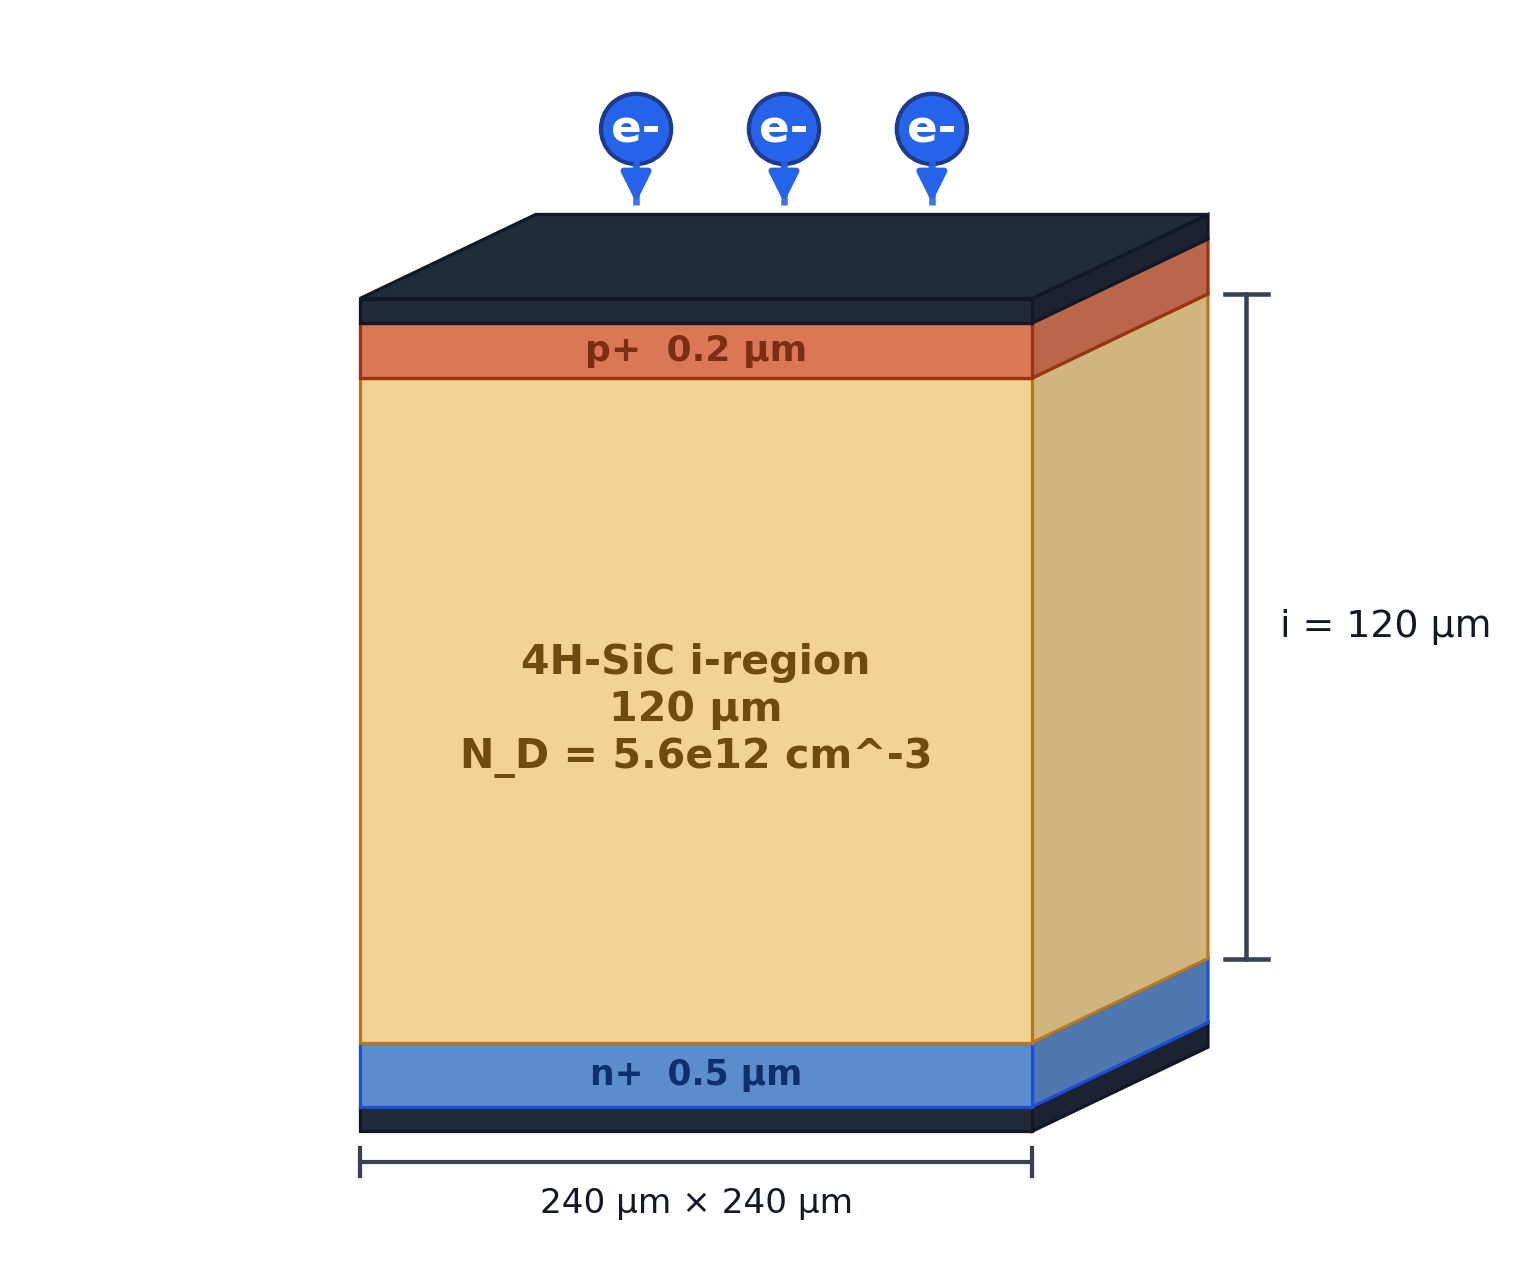
\includegraphics[keepaspectratio,alt={Fig.1 4H-SiC PIN 探测器结构示意图}]{figures/fig1_sic_pin_structure.png}}

\textbf{Fig.1.} 4H-SiC PIN 探测器结构示意图。图中以
\(W_i=120\ \mu\mathrm{m}\) 为参考结构展示，本文实际扫描
\(W_i=5\)、8、10-130、150 和 \(180\ \mu\mathrm{m}\)。

\textbf{Table 2. 器件结构和材料参数。}

{\def\LTcaptype{none} % do not increment counter
\begin{longtable}[]{@{}lr@{}}
\toprule\noalign{}
参数 & 数值 \\
\midrule\noalign{}
\endhead
\bottomrule\noalign{}
\endlastfoot
\(p^+\) 厚度 & \(0.2\ \mu\mathrm{m}\) \\
i 区厚度 & 5、8、10-130、150、\(180\ \mu\mathrm{m}\) \\
\(n^+\) 厚度 & \(0.5\ \mu\mathrm{m}\) \\
横向尺寸 & \(240\ \mu\mathrm{m}\times240\ \mu\mathrm{m}\) \\
i 区净掺杂 & \(5.6\times10^{12}\ \mathrm{cm^{-3}}\) \\
p+ / n+ 掺杂 & \(1\times10^{19}\ \mathrm{cm^{-3}}\) \\
\end{longtable}
}

对于每个 \(W_i\)，工作偏压取对应全耗尽偏压。耗尽电压的解析估算为

\[
V_{\mathrm{dep}}(W_i)=\frac{qN_DW_i^2}{2\varepsilon_{\mathrm{SiC}}}.
\]

Sentaurus 中的电势、电场和载流子输运由 Poisson
方程和漂移扩散方程自洽求解。全耗尽偏压用于保证不同厚度器件在可比的收集条件下评估
CCE。

\subsubsection{2.2 Geant4 能量沉积与 TCAD
映射}\label{geant4-ux80fdux91cfux6c89ux79efux4e0e-tcad-ux6620ux5c04}

Geant4 用于模拟 C-14 β 电子和单能电子在 4H-SiC
中的输运与能量沉积。电磁相互作用采用适用于 keV 电子的低能电磁模型。C-14
源项按照理论 β 谱采样，最大能量为 156.5 keV，平均能量约为 49
keV。对照单能源项选择 20、49、100 和 156.5 keV。Geant4
输出的能量沉积先统计为深度分布 \(dE/dz\)，再转换为二维载流子生成率分布
\(G(x,y)\)。

\pandocbounded{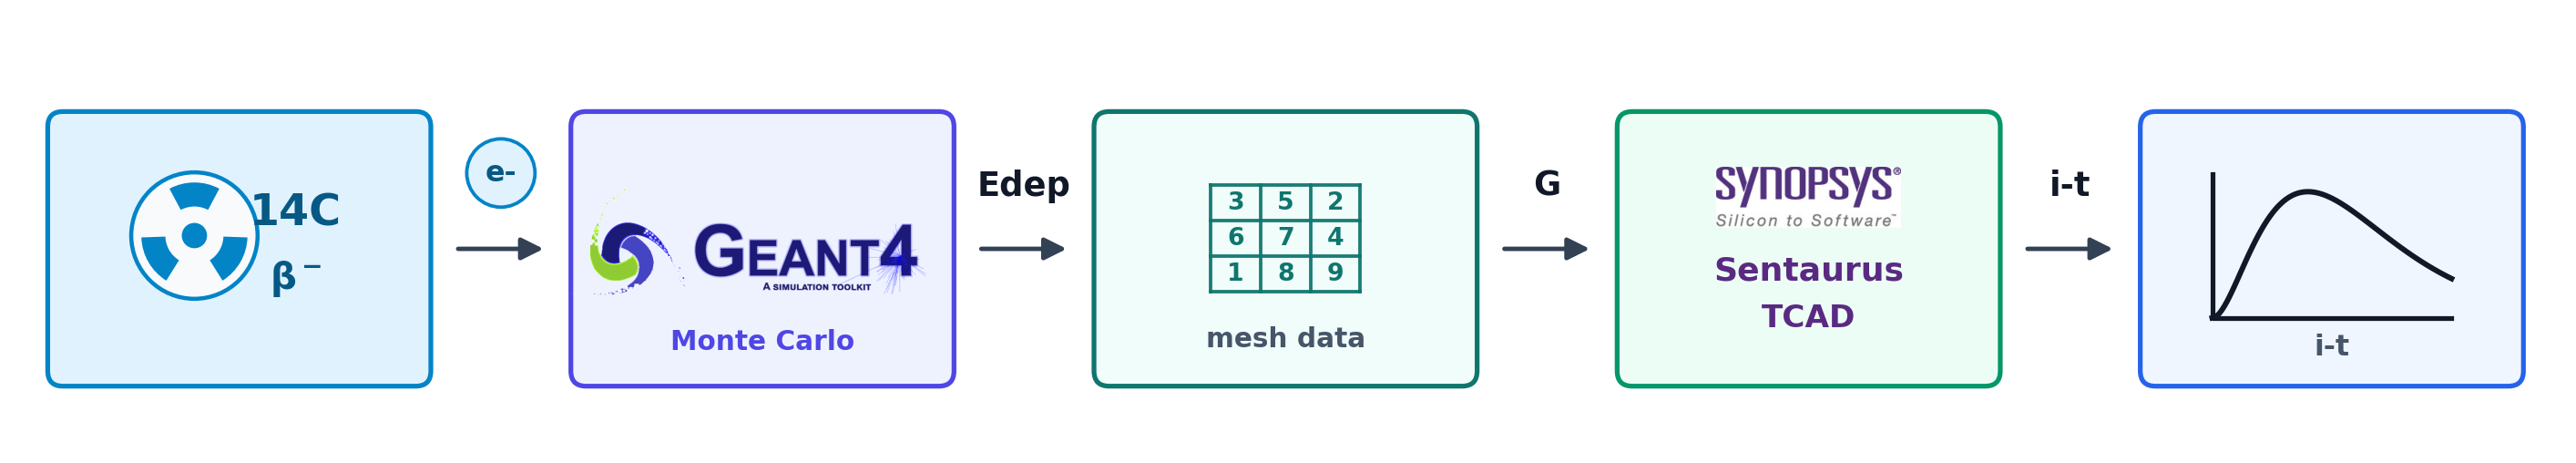
\includegraphics[keepaspectratio,alt={Fig.2 Geant4-Sentaurus 耦合仿真流程}]{figures/fig2_geant4_tcad_workflow.png}}

\textbf{Fig.2.} Geant4-Sentaurus 耦合仿真流程。Geant4 端给出 β 电子在
4H-SiC 中的能量沉积分布，后处理程序将其转换为电子-空穴对生成率并映射至
Sentaurus 网格，最终通过瞬态电流积分得到 CCE。

能量沉积到载流子产生量的转换采用 4H-SiC 平均电子-空穴对产生能量
\(E_{eh}=7.8\ \mathrm{eV}\)：

\[
N_{eh}=\frac{E_{\mathrm{dep}}}{E_{eh}}.
\]

由于 Geant4 统计网格与 Sentaurus
非均匀器件网格不完全重合，本文采用双线性插值进行空间映射。对任意
Sentaurus 网格点 \((x,y)\)，在 Geant4
转换后的二维生成率网格中找到包围该点的四个相邻节点，并按

\[
G(x,y)=(1-t)(1-u)G_{11}+t(1-u)G_{21}+(1-t)uG_{12}+tuG_{22}
\]

计算该点处的生成率。这里
\(t=(x-x_1)/(x_2-x_1)\)，\(u=(y-y_1)/(y_2-y_1)\)。

尽管入射方向为垂直方向，keV 电子在 SiC
中仍会发生多次散射，且低能电子的横向展宽与近表面沉积位置有关。因此，本文保留
Geant4
输出的二维沉积分布，而不是先做横向平均后再映射。为降低统计涨落影响，后处理阶段对沉积网格进行归一化并检查总沉积能量守恒；Fig.2(b)
给出了映射后的典型二维生成率分布。该处理的目标是保持 Geant4
横向散射信息与 Sentaurus
非均匀网格的一致性，而不是引入额外的横向物理假设。

\pandocbounded{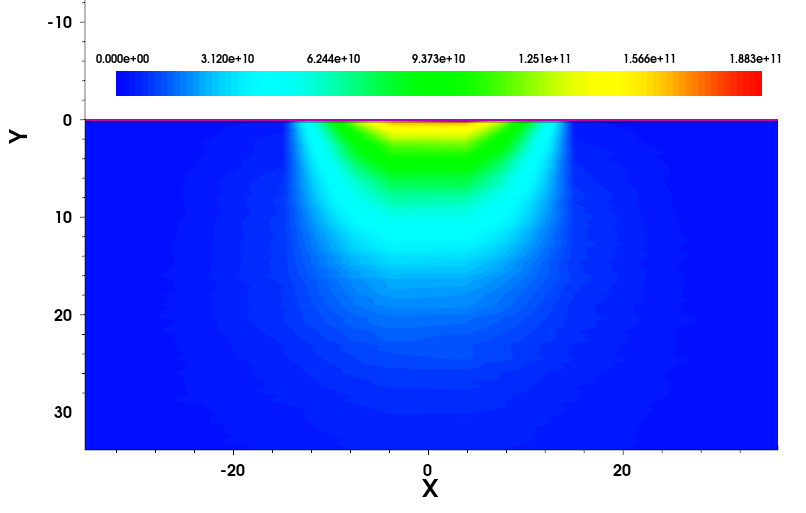
\includegraphics[keepaspectratio,alt={Fig.2b Sentaurus/TDR 网格中的载流子生成率分布}]{figures/fig2b_tdr_generation_distribution.png}}

\textbf{Fig.2(b).} Sentaurus/TDR
网格中的载流子生成率分布示例。生成率在横向和深度方向均存在明显梯度，说明
Geant4 能量沉积分布已经被映射到 TCAD 器件区域中。

\subsubsection{2.3 Sentaurus
物理模型}\label{sentaurus-ux7269ux7406ux6a21ux578b}

TCAD 仿真求解 Poisson
方程与电子、空穴连续性方程。载流子输运采用漂移扩散模型，并考虑 4H-SiC
各向异性迁移率、掺杂依赖迁移率、高场饱和和不完全电离。复合模型采用 SRH
形式。对有缺陷材料，Z1/2 和 EH6/7 深能级以体缺陷形式加入 i 区。

瞬态仿真输出阴极电流
\(i_{\mathrm{cathode}}(t)\)。本文不再将瞬态波形宽度作为优化指标，而仅将
\(i(t)\) 用于电荷积分和 CCE 计算。

\subsubsection{2.4
外延层固有缺陷模型}\label{ux5916ux5ef6ux5c42ux56faux6709ux7f3aux9677ux6a21ux578b}

本文关注外延层固有缺陷对器件设计的影响，而不是特定辐照历史下的损伤演化。Z1/2
和 EH6/7 是 n 型或轻掺杂 4H-SiC
外延层中常见的碳空位相关深能级，并被广泛认为会限制少子寿命和电荷收集性能
{[}16{]}-{[}18{]}。本文采用文献约束的两中心 SRH 体缺陷模型，参数列于
Table 3。\(N_t\) 表示每一类缺陷中心在 i 区中的均匀体浓度，即
\(N_{\mathrm{Z1/2}}=N_{\mathrm{EH6/7}}=N_t\)。

\textbf{Table 3. TCAD 仿真采用的 SRH 体陷阱参数。}

{\def\LTcaptype{none} % do not increment counter
\begin{longtable}[]{@{}
  >{\raggedright\arraybackslash}p{(\linewidth - 12\tabcolsep) * \real{0.1250}}
  >{\raggedright\arraybackslash}p{(\linewidth - 12\tabcolsep) * \real{0.1250}}
  >{\raggedright\arraybackslash}p{(\linewidth - 12\tabcolsep) * \real{0.1250}}
  >{\raggedleft\arraybackslash}p{(\linewidth - 12\tabcolsep) * \real{0.1667}}
  >{\raggedleft\arraybackslash}p{(\linewidth - 12\tabcolsep) * \real{0.1667}}
  >{\raggedleft\arraybackslash}p{(\linewidth - 12\tabcolsep) * \real{0.1667}}
  >{\raggedright\arraybackslash}p{(\linewidth - 12\tabcolsep) * \real{0.1250}}@{}}
\toprule\noalign{}
\begin{minipage}[b]{\linewidth}\raggedright
Center
\end{minipage} & \begin{minipage}[b]{\linewidth}\raggedright
TCAD type
\end{minipage} & \begin{minipage}[b]{\linewidth}\raggedright
Energy level
\end{minipage} & \begin{minipage}[b]{\linewidth}\raggedleft
\(\sigma_e\) (cm\(^2\))
\end{minipage} & \begin{minipage}[b]{\linewidth}\raggedleft
\(\sigma_h\) (cm\(^2\))
\end{minipage} & \begin{minipage}[b]{\linewidth}\raggedleft
Concentration
\end{minipage} & \begin{minipage}[b]{\linewidth}\raggedright
Main basis
\end{minipage} \\
\midrule\noalign{}
\endhead
\bottomrule\noalign{}
\endlastfoot
Z1/2 & Acceptor & \(E_c-0.67\ \mathrm{eV}\) & \(2\times10^{-14}\) &
\(1\times10^{-15}\) & \(N_t\) & Z1/2 level and acceptor assignment from
TCAD/DLTS studies {[}17{]}, {[}18{]}; \(\sigma_e\) follows reported TCAD
values {[}17{]}, {[}19{]} \\
EH6/7 & Donor & \(E_c-1.55\ \mathrm{eV}\) & \(2\times10^{-14}\) &
\(1\times10^{-15}\) & \(N_t\) & EH6/7 DLTS energies fall near 1.49-1.63
eV {[}16{]}; donor assignment and TCAD use from {[}17{]}; capture cross
sections chosen within reported TCAD/DLTS order of magnitude {[}16{]},
{[}19{]} \\
\end{longtable}
}

Z1/2 的能级和电子俘获截面直接采用 Gaggl 等 TCAD 缺陷模型中的取值
{[}17{]}。EH6/7 能级取 Kleppinger 等 DLTS 提取范围 1.49-1.63 eV
内的代表值，并接近 Gaggl 等辐照损伤 TCAD 模型采用的
\(E_c-1.60\ \mathrm{eV}\) {[}16{]},
{[}17{]}。由于文献报道的俘获截面会随材料、提取方法和校准目标发生明显变化，本文固定
\(\sigma_e\) 和 \(\sigma_h\)，将 \(N_t\)
作为受控材料质量参数。等浓度条件
\(N_{\mathrm{Z1/2}}=N_{\mathrm{EH6/7}}=N_t\)
是设计空间假设，而不是对某一外延片 DLTS
谱的拟合。该处理把两类中心的相对浓度和截面不确定性折合进单一等效体陷阱密度，因此本文给出的
\(N_t\) 不应被解释为唯一的材料表征量。若真实外延层中 Z1/2 与 EH6/7
的比例显著偏离
1:1，最优厚度的绝对数值可能发生移动；但只要深层俘获概率随漂移距离增加而增强，缺陷升高导致厚端
CCE 下降、最优厚度向薄端回缩的趋势仍然成立。后续需要通过 DLTS
或寿命数据校准各中心浓度，并对 \(\sigma_e\)、\(\sigma_h\)
进行敏感性分析。

扫描的缺陷密度为

\[
N_t = 0,\ 10^{12},\ 10^{13},\ 2.5\times10^{13},\ 5\times10^{13}\ \mathrm{cm^{-3}}.
\]

其中 \(N_t=0\) 作为理想材料基线，\(10^{12}\ \mathrm{cm^{-3}}\)
表示低缺陷或高质量外延层情形，\(10^{13}\ \mathrm{cm^{-3}}\)
表示缺陷较丰富的外延层情形，\(2.5\times10^{13}\) 和
\(5\times10^{13}\ \mathrm{cm^{-3}}\)
用于表示更严重的缺陷或等效退化上限情形。由于本文目标是建立厚度选择设计图，而不是反演某一批外延片的真实
DLTS 谱，\(N_t\) 应理解为等效体陷阱密度，而非对商业外延材料的绝对分级。

\subsubsection{2.5 CCE 计算}\label{cce-ux8ba1ux7b97}

本文采用 CCE 作为唯一品质因子：

\[
\mathrm{CCE}=\frac{Q_{\mathrm{collected}}}{Q_{\mathrm{generated}}}\times100\%.
\]

其中

\[
Q_{\mathrm{collected}}=\int_0^{T_{\mathrm{int}}}i_{\mathrm{cathode}}(t)\,dt,
\]

而

\[
Q_{\mathrm{generated}}=\frac{E_{\mathrm{dep}}}{E_{eh}}q.
\]

这里的 \(E_{\mathrm{dep}}\) 指 Geant4 后处理后被映射到 TCAD
载流子产生分布中的沉积能量，而不是入射 β
粒子的全部初始能量。因此，本文的 CCE
是相对于``已在器件模型中产生的电子-空穴对''的收集效率，不等同于总探测效率或能量吸收效率。p+
入射层、近表面复合和穿透出器件后的未沉积能量会影响真实探测效率，但不计入本文
CCE 分母。Fano
因子主要影响能量分辨率和脉冲高度谱展宽；本文不以能谱重建为优化目标，因此未将其纳入
CCE 计算。

选择 CCE
作为单一目标量的原因是，本文的核心问题是给定外延材料质量后如何选择 i
区厚度以最大化有效收集电荷。缺陷俘获和复合的直接结果是积分收集电荷下降，因此
CCE 比瞬态波形形状更适合作为厚度优化目标。换言之，本文研究对象是 C-14 β
探测器的结构设计，而不是完整 β 谱仪的能量分辨率优化。

\subsection{3. 结果}\label{ux7ed3ux679c}

\subsubsection{3.1 C-14 β
谱和能量沉积分布}\label{c-14-ux3b2-ux8c31ux548cux80fdux91cfux6c89ux79efux5206ux5e03}

Fig.3 给出 C-14 理论 β 谱和 Geant4 采样结果。C-14 β 谱覆盖从近零到 156.5
keV 的连续能量区间，不能由单一能量点完整表示。

\pandocbounded{
\includegraphics[keepaspectratio,alt={Fig.3 C-14 β 能谱}]{figures/fig3_c14_spectrum.png}}

\textbf{Fig.3.} C-14 β 能谱及 Geant4 采样结果。平均能量约为 49
keV，最大能量为 156.5 keV。

Fig.4 比较了 C-14 连续谱与多个单能源项在 4H-SiC 中的深度能量沉积分布。20
keV 电子主要在近表面区域沉积；49 keV 接近 C-14
平均能量，但只能代表有限深度范围；100 和 156.5 keV
电子具有更深穿透尾部。C-14
连续谱则叠加了浅层沉积和高能尾部，空间分布明显不同于任一单能源项。

\pandocbounded{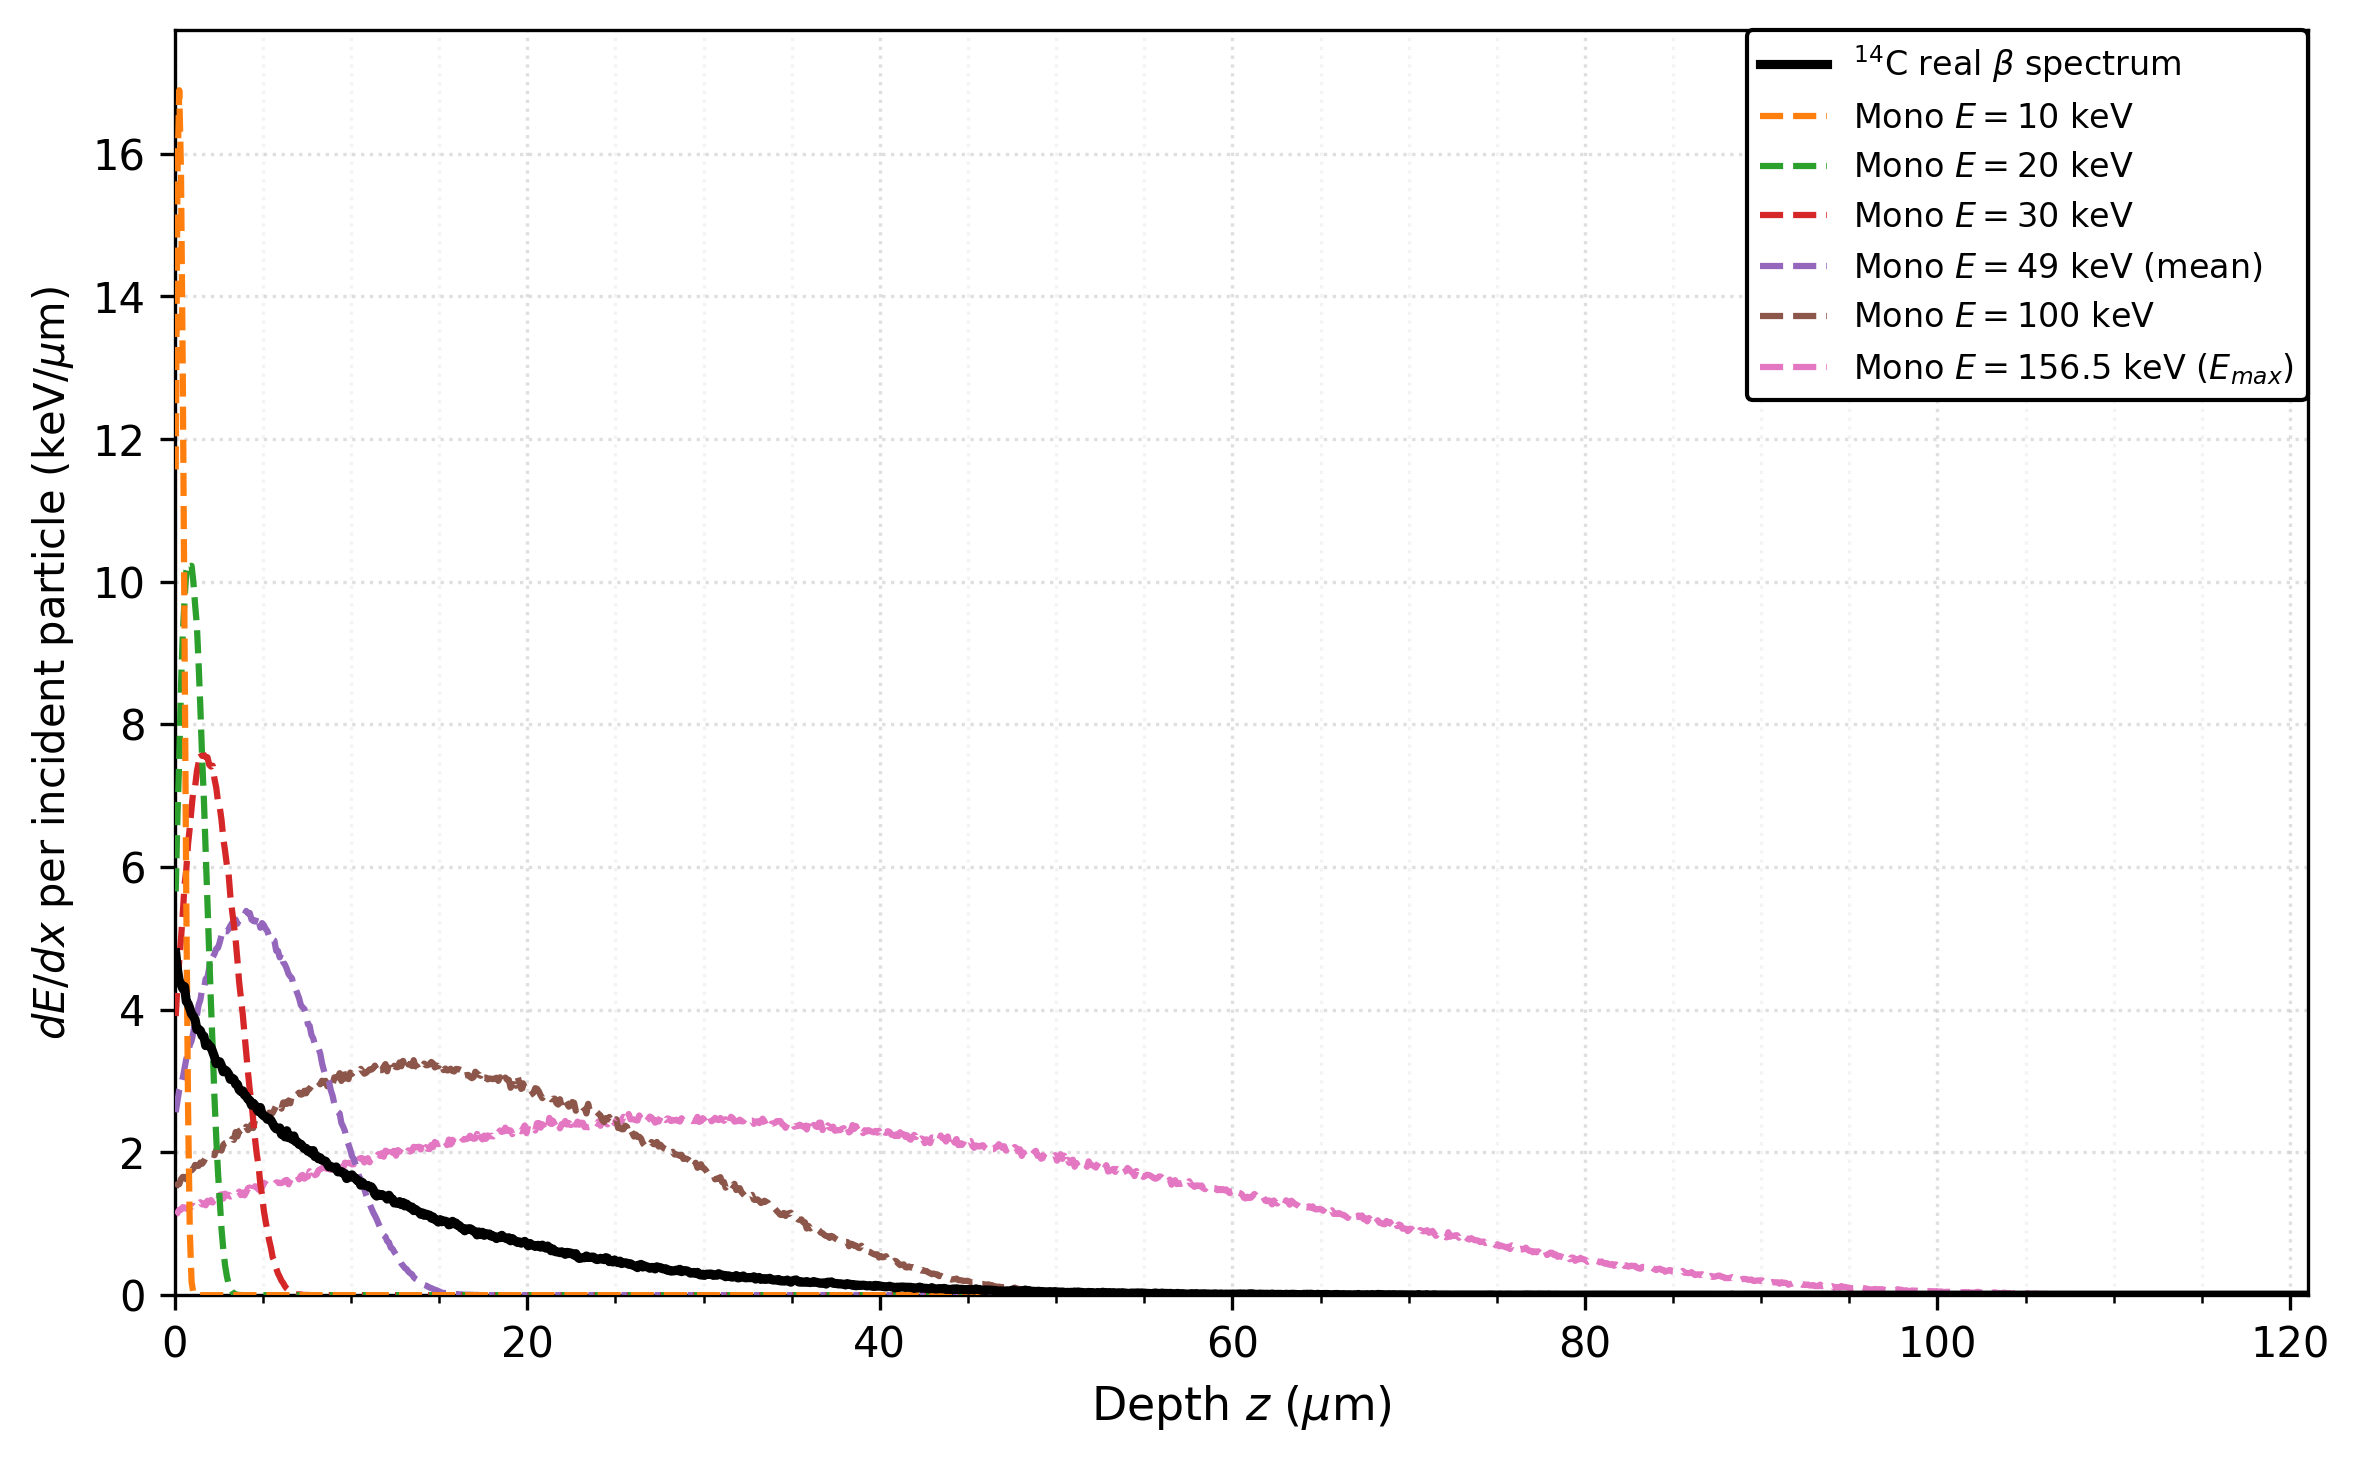
\includegraphics[keepaspectratio,alt={Fig.4 不同源项在 4H-SiC 中的深度能量沉积分布}]{figures/fig4_dedx_profiles.png}}

\textbf{Fig.4.} 不同源项在 4H-SiC
中的深度能量沉积分布。主文后续厚度优化选取 20、49、100、156.5 keV 和
C-14 连续谱作为对照源项。

这一结果说明，若使用平均能量 49 keV 代表 C-14 谱，将低估高能尾部对较厚 i
区的需求；若使用 156.5 keV 代表 C-14
谱，则会过度强调极高能端粒子并可能导致过厚设计。

\subsubsection{3.2
器件电学表征}\label{ux5668ux4ef6ux7535ux5b66ux8868ux5f81}

在进行 CCE 设计扫描前，需要确认 TCAD
器件模型在基准工作点附近已经进入全耗尽状态。Fig.5 给出
\(W_i=120\ \mu\mathrm{m}\) baseline 4H-SiC PIN 器件的 C-V
特性，其中主图采用 \(1/C^2\)-V 形式，inset 给出原始 C-V 曲线。采用
\(1/C^2\)-V
是因为该表示方式能够更清楚地展示反偏增大时耗尽层扩展并逐渐进入平台的过程；原始
C-V inset 则用于直观显示电容随反偏升高而下降并接近几何电容。

\pandocbounded{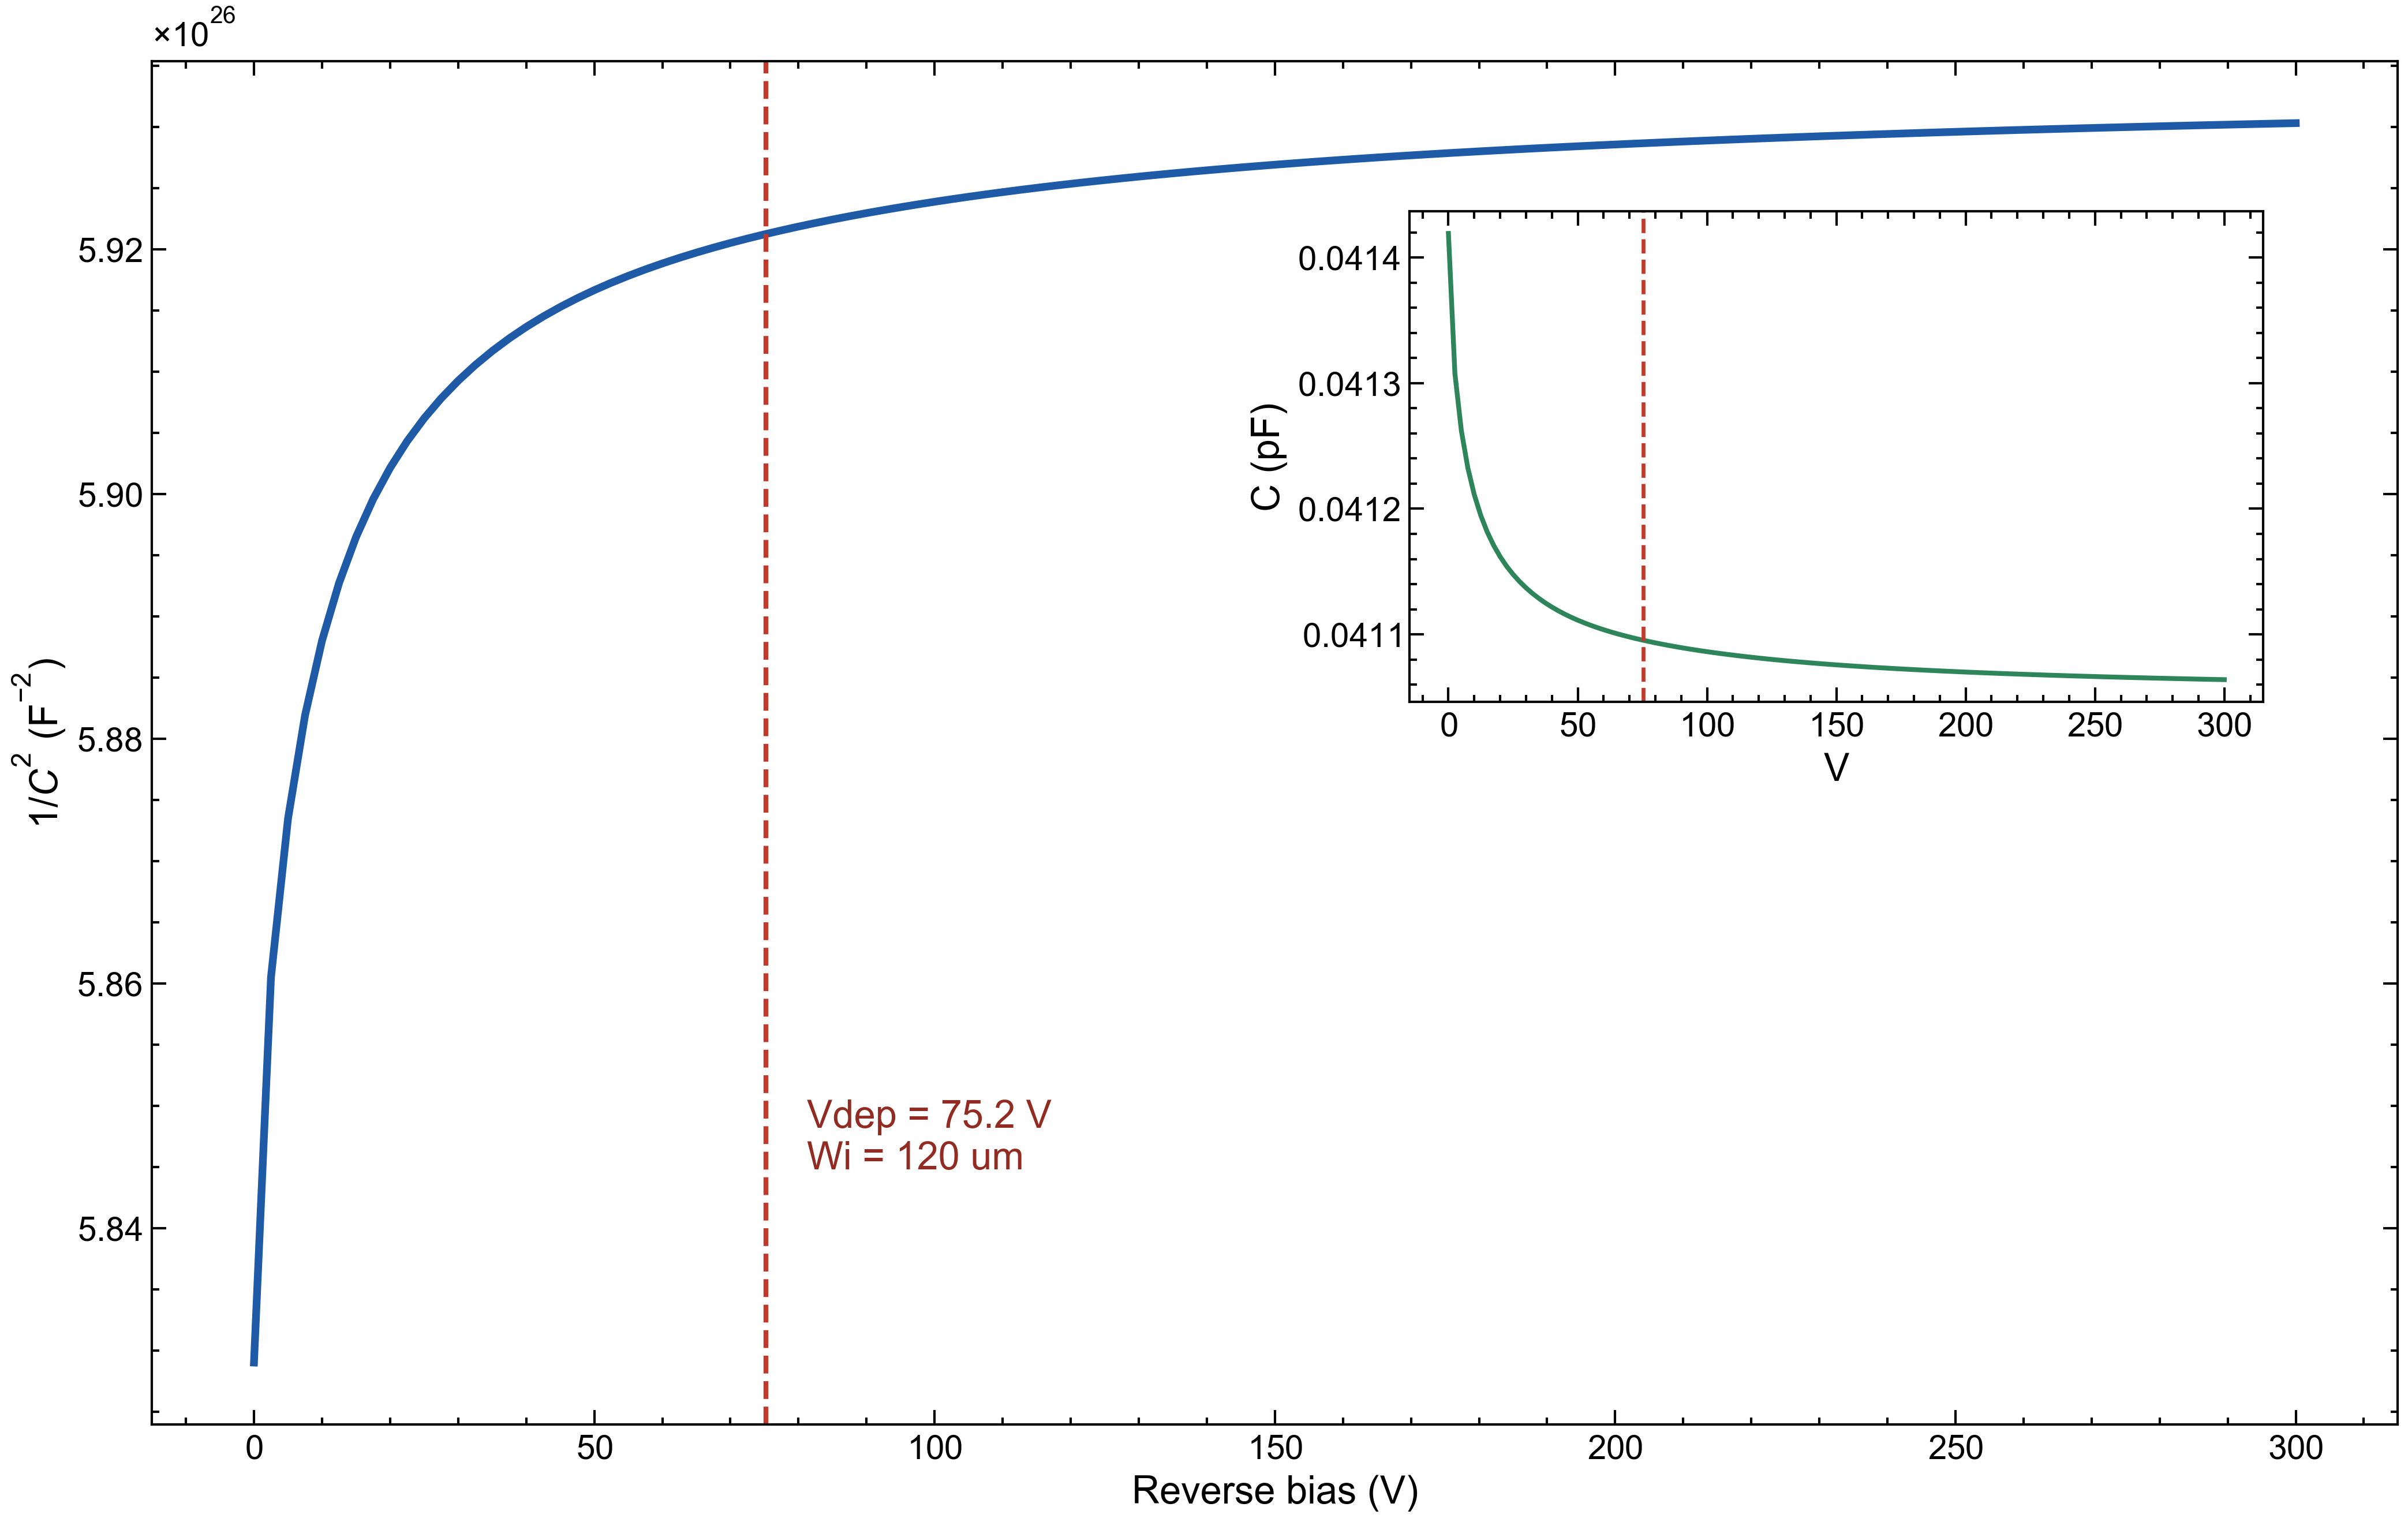
\includegraphics[keepaspectratio,alt={Fig.5 baseline 器件 1/C²-V 与 C-V 特性}]{figures/fig5_cv_1overc2_baseline.png}}

\textbf{Fig.5.} \(W_i=120\ \mu\mathrm{m}\) baseline 4H-SiC PIN 器件的
\(1/C^2\)-V 特性，inset 为原始 C-V
曲线。竖直虚线标出由一维耗尽近似得到的全耗尽电压。

对于本文的 baseline 器件，i 区净掺杂为
\(N_D=5.6\times10^{12}\ \mathrm{cm^{-3}}\)，厚度为
\(W_i=120\ \mu\mathrm{m}\)。由

\[
V_{\mathrm{dep}}=\frac{qN_DW_i^2}{2\varepsilon_{\mathrm{SiC}}}
\]

计算得到的全耗尽电压为 75.2 V。Fig.5 中 \(1/C^2\)
随反偏升高快速增加，并在该电压之后逐渐趋于高反偏平台；inset 中的 C-V
曲线也显示电容从 \(4.14\times10^{-14}\) F 下降并接近
\(4.11\times10^{-14}\) F 的几何电容水平。因此，后续以 75 V 作为
\(120\ \mu\mathrm{m}\) baseline 器件的瞬态仿真偏压是合理的。

\subsubsection{3.3 缺陷对 C-14
CCE-厚度关系的影响}\label{ux7f3aux9677ux5bf9-c-14-cce-ux539aux5ea6ux5173ux7cfbux7684ux5f71ux54cd}

Fig.6 给出 C-14 连续谱下 CCE 随 i 区厚度和体缺陷密度 \(N_t\)
的变化。完整数据覆盖 5 个源项、17 个厚度和 5 个缺陷密度，共 425 个 TCAD
瞬态响应组合；本节选取其中 C-14
连续谱结果作为主线分析对象。每条瞬态电流曲线均按相同积分窗口计算收集电荷，并进一步归一化为
CCE。

\pandocbounded{
\includegraphics[keepaspectratio,alt={Fig.6 C-14 谱下 CCE 随 i 区厚度和缺陷密度的变化}]{figures/fig6_c14_cce_vs_thickness_by_Nt.png}}

\textbf{Fig.6.} C-14 连续谱下 CCE 随 i
区厚度变化的曲线族，参数为陷阱密度 \(N_t\)。低缺陷密度下 CCE
随厚度增加后趋于饱和；高缺陷密度下厚端俘获损失增强，CCE 变为非单调函数。

理想材料和低缺陷材料中，CCE 从薄端快速上升，并在
\(W_i\approx100\ \mu\mathrm{m}\)
后进入接近饱和的区域。\(N_t=10^{12}\ \mathrm{cm^{-3}}\)
的曲线几乎与理想材料重合，说明高质量外延层中陷阱俘获不是限制 C-14
电荷收集的主导因素。随着 \(N_t\) 增加到
\(10^{13}\ \mathrm{cm^{-3}}\)，厚器件中的 CCE
开始明显下降，最优厚度回缩到 \(60\ \mu\mathrm{m}\)；当
\(N_t=2.5\times10^{13}\) 和 \(5\times10^{13}\ \mathrm{cm^{-3}}\) 时，CCE
分别在 40 和 \(30\ \mu\mathrm{m}\)
附近达到最大值，随后随厚度增加而持续降低。

这一现象可以由两个竞争机制解释。薄端 CCE 受限于 C-14
高能尾部的能量沉积覆盖率，增加厚度有利于提高可收集电荷。厚端 CCE
则受限于深处载流子的漂移距离和陷阱俘获概率，增加厚度会放大缺陷引起的收集损失。两种机制竞争后，CCE
从理想材料中的单调饱和函数转变为高缺陷材料中的非单调函数，最优 i
区厚度因此自然出现。

完整数据给出的 C-14 最优设计点如下。

\textbf{Table 4. C-14 连续谱下以 CCE 最大化得到的最优设计点。}

{\def\LTcaptype{none} % do not increment counter
\begin{longtable}[]{@{}
  >{\raggedleft\arraybackslash}p{(\linewidth - 8\tabcolsep) * \real{0.2105}}
  >{\raggedleft\arraybackslash}p{(\linewidth - 8\tabcolsep) * \real{0.2105}}
  >{\raggedleft\arraybackslash}p{(\linewidth - 8\tabcolsep) * \real{0.2105}}
  >{\raggedleft\arraybackslash}p{(\linewidth - 8\tabcolsep) * \real{0.2105}}
  >{\raggedright\arraybackslash}p{(\linewidth - 8\tabcolsep) * \real{0.1579}}@{}}
\toprule\noalign{}
\begin{minipage}[b]{\linewidth}\raggedleft
\(N_t\) (cm\(^{-3}\))
\end{minipage} & \begin{minipage}[b]{\linewidth}\raggedleft
最优 \(W_i\) (\(\mu\)m)
\end{minipage} & \begin{minipage}[b]{\linewidth}\raggedleft
偏压 (V)
\end{minipage} & \begin{minipage}[b]{\linewidth}\raggedleft
最优 CCE (\%)
\end{minipage} & \begin{minipage}[b]{\linewidth}\raggedright
说明
\end{minipage} \\
\midrule\noalign{}
\endhead
\bottomrule\noalign{}
\endlastfoot
0 & 150 & 117 & 97.80 & 理想材料，厚端饱和区内最高点 \\
\(10^{12}\) & 100 & 52 & 97.72 & 低缺陷外延层，厚端仍有效 \\
\(10^{13}\) & 60 & 19 & 95.09 & 缺陷俘获使最优厚度回缩 \\
\(2.5\times10^{13}\) & 40 & 8 & 87.14 & 高缺陷条件下厚端损失显著 \\
\(5\times10^{13}\) & 30 & 5 & 81.72 & 严重缺陷条件下薄 i 区更优 \\
\end{longtable}
}

\subsubsection{3.4 C-14 CCE
设计地图}\label{c-14-cce-ux8bbeux8ba1ux5730ux56fe}

Fig.7 将 C-14 连续谱下的 CCE 结果整理为离散设计地图。横轴选取
30、40、60、100 和 \(150\ \mu\mathrm{m}\) 五个代表性 i
区厚度，纵轴为陷阱密度 \(N_t\)，每个格子的颜色和数字表示对应设计点的
CCE，颜色越深表示 CCE 越高。该表示方式可以直接显示高 CCE
设计区域如何随缺陷密度变化而移动。

\pandocbounded{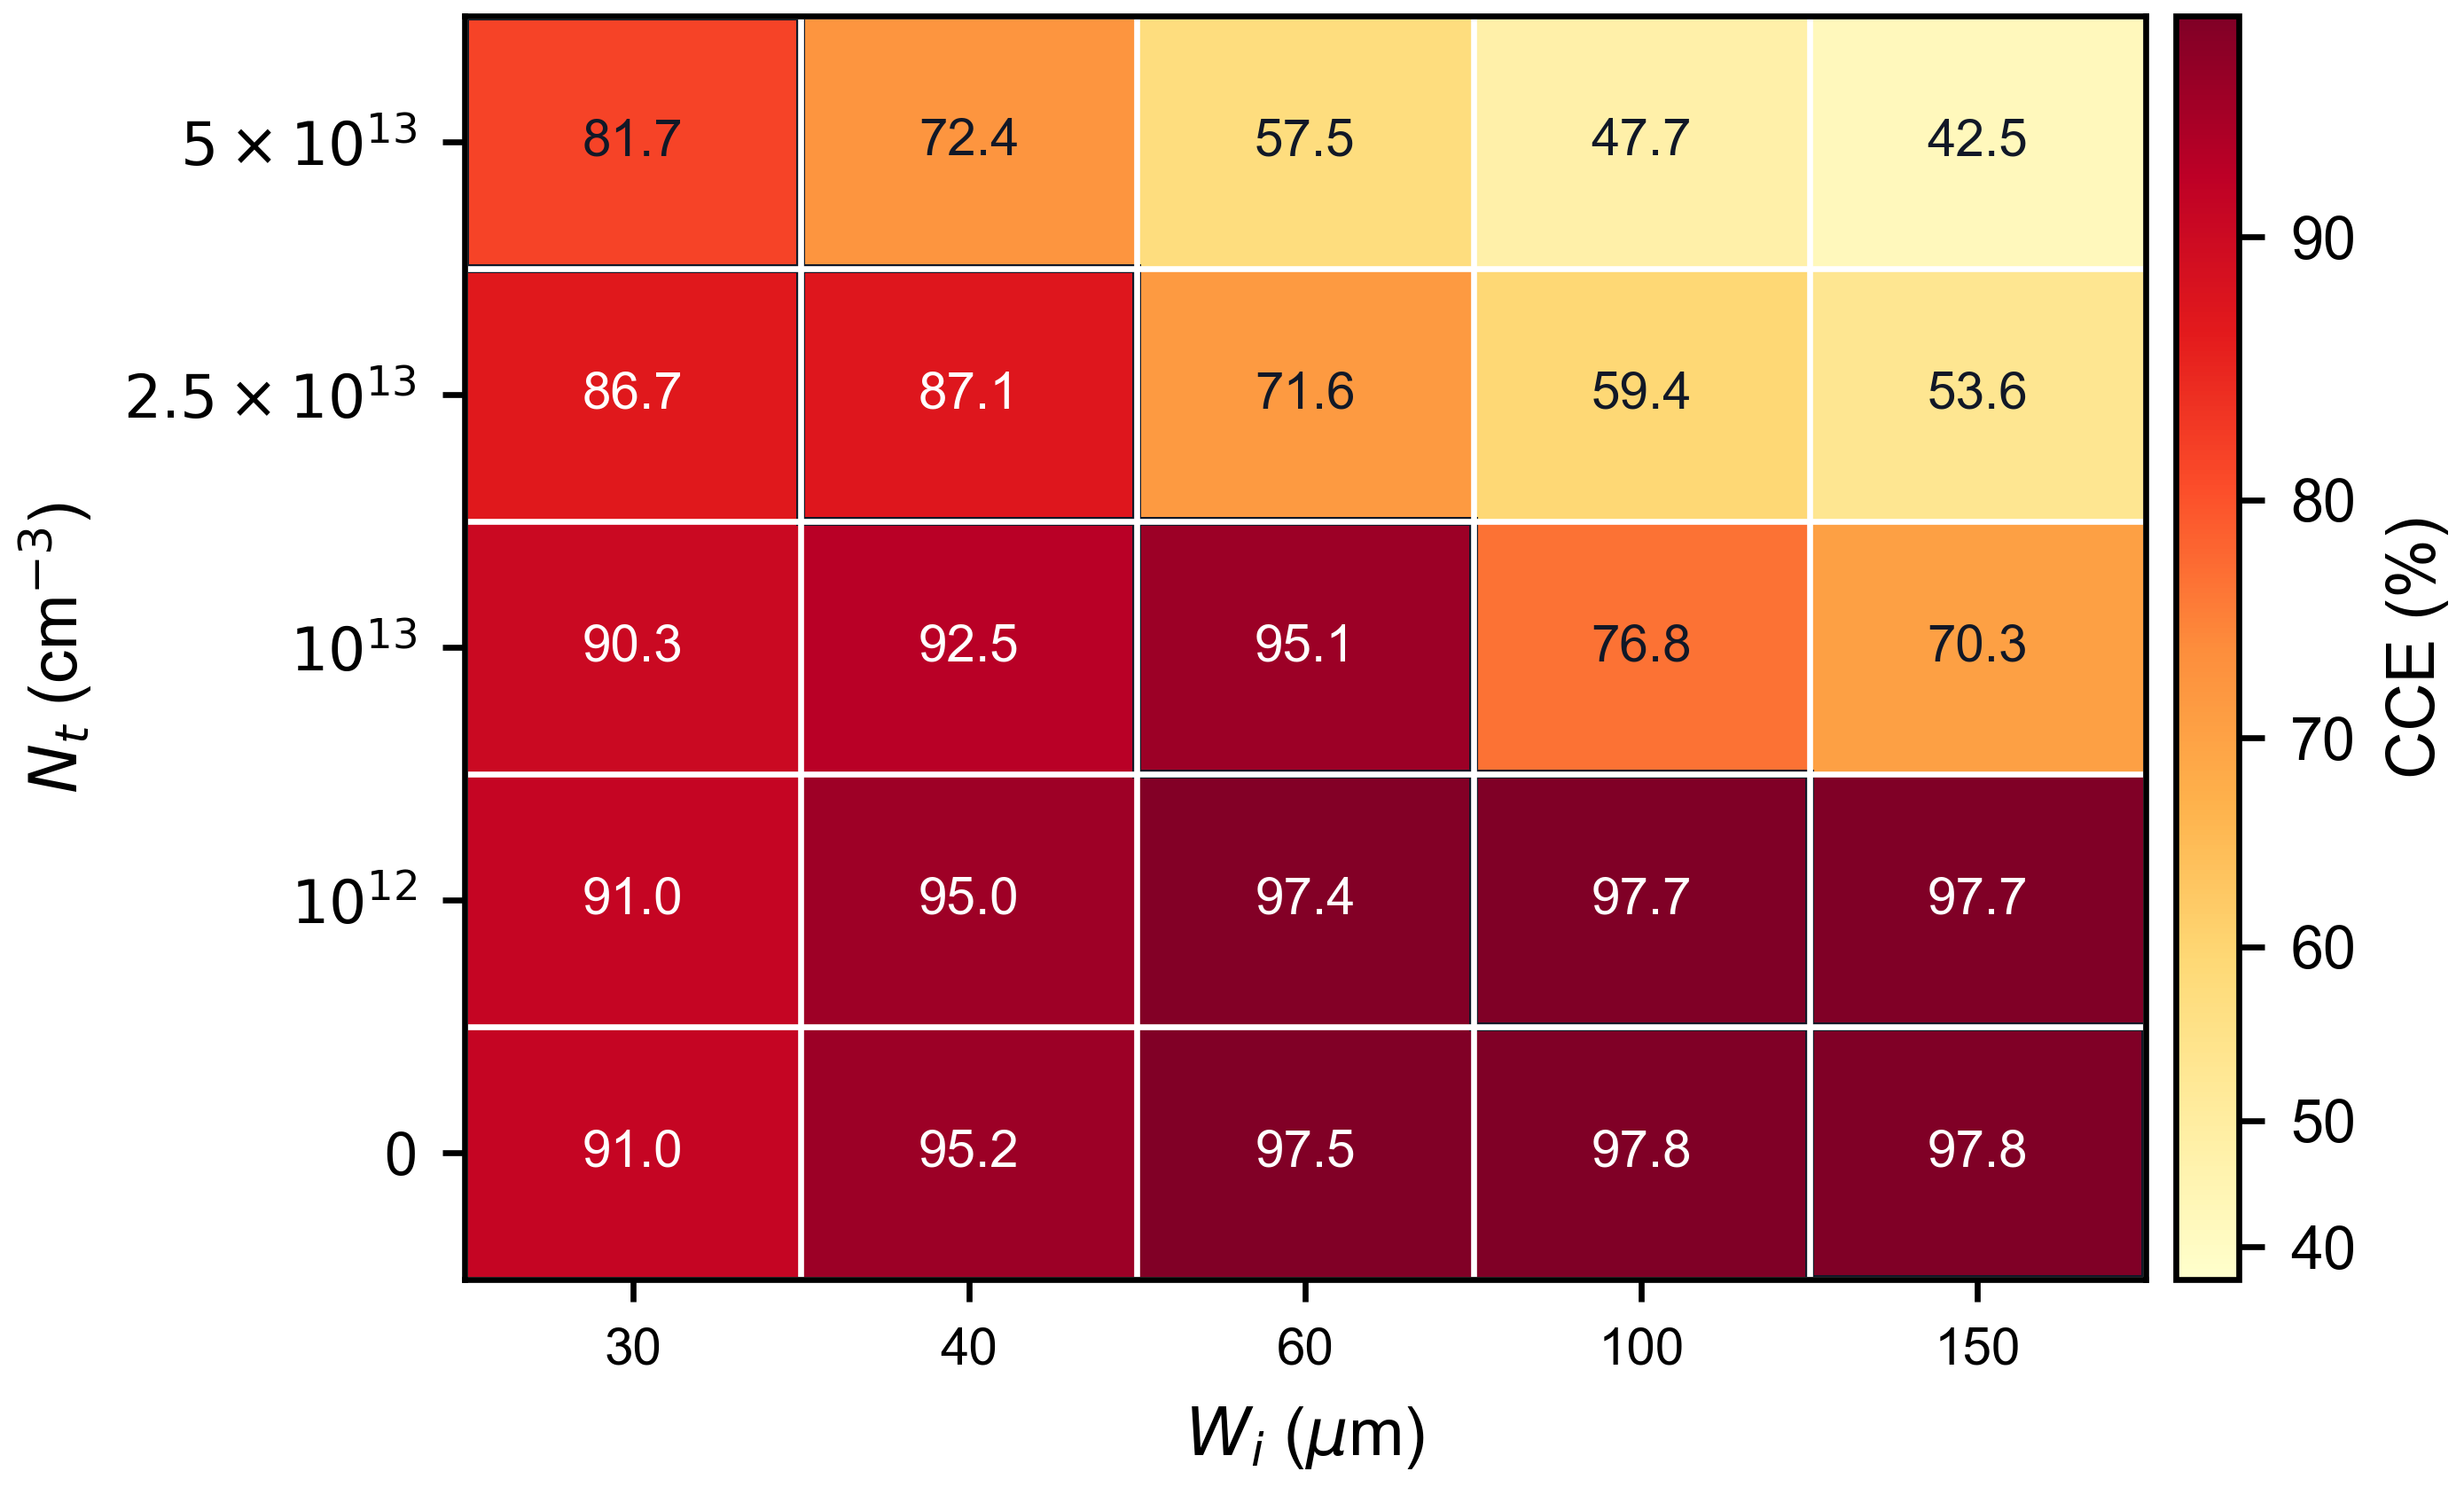
\includegraphics[keepaspectratio,alt={Fig.7 C-14 CCE 设计地图}]{figures/fig7_c14_cce_design_map.png}}

\textbf{Fig.7.} C-14 连续谱下 CCE 关于代表性 i 区厚度和陷阱密度 \(N_t\)
的离散设计地图。横向每一列对应一个代表厚度，纵向每一行对应一个缺陷密度，颜色越深表示
CCE 越高；黑框标出该缺陷密度下五个代表厚度中的最高 CCE。

在 \(N_t=0\) 和 \(10^{12}\ \mathrm{cm^{-3}}\) 时，高 CCE 区域覆盖
100-\(150\ \mu\mathrm{m}\)
的厚端代表点，说明低缺陷材料中厚度选择具有较宽容差。随着 \(N_t\) 增加到
\(10^{13}\ \mathrm{cm^{-3}}\)，厚端格子明显变浅，高 CCE 区域集中到
\(60\ \mu\mathrm{m}\)。进一步增加到 \(2.5\times10^{13}\) 和
\(5\times10^{13}\ \mathrm{cm^{-3}}\) 后，高 CCE 区域继续向 40 和
\(30\ \mu\mathrm{m}\) 回缩，而 \(100\ \mu\mathrm{m}\)
以上厚端区域出现显著收集损失。

\subsubsection{3.5
推广到单能源项的最优厚度}\label{ux63a8ux5e7fux5230ux5355ux80fdux6e90ux9879ux7684ux6700ux4f18ux539aux5ea6}

为了比较单能源项与 C-14 连续谱，本文在 20、49、100、156.5 keV 和 C-14
五个源项下分别计算使 CCE 最大化的 i 区厚度。Fig.8 给出最优厚度随 \(N_t\)
的变化。

\pandocbounded{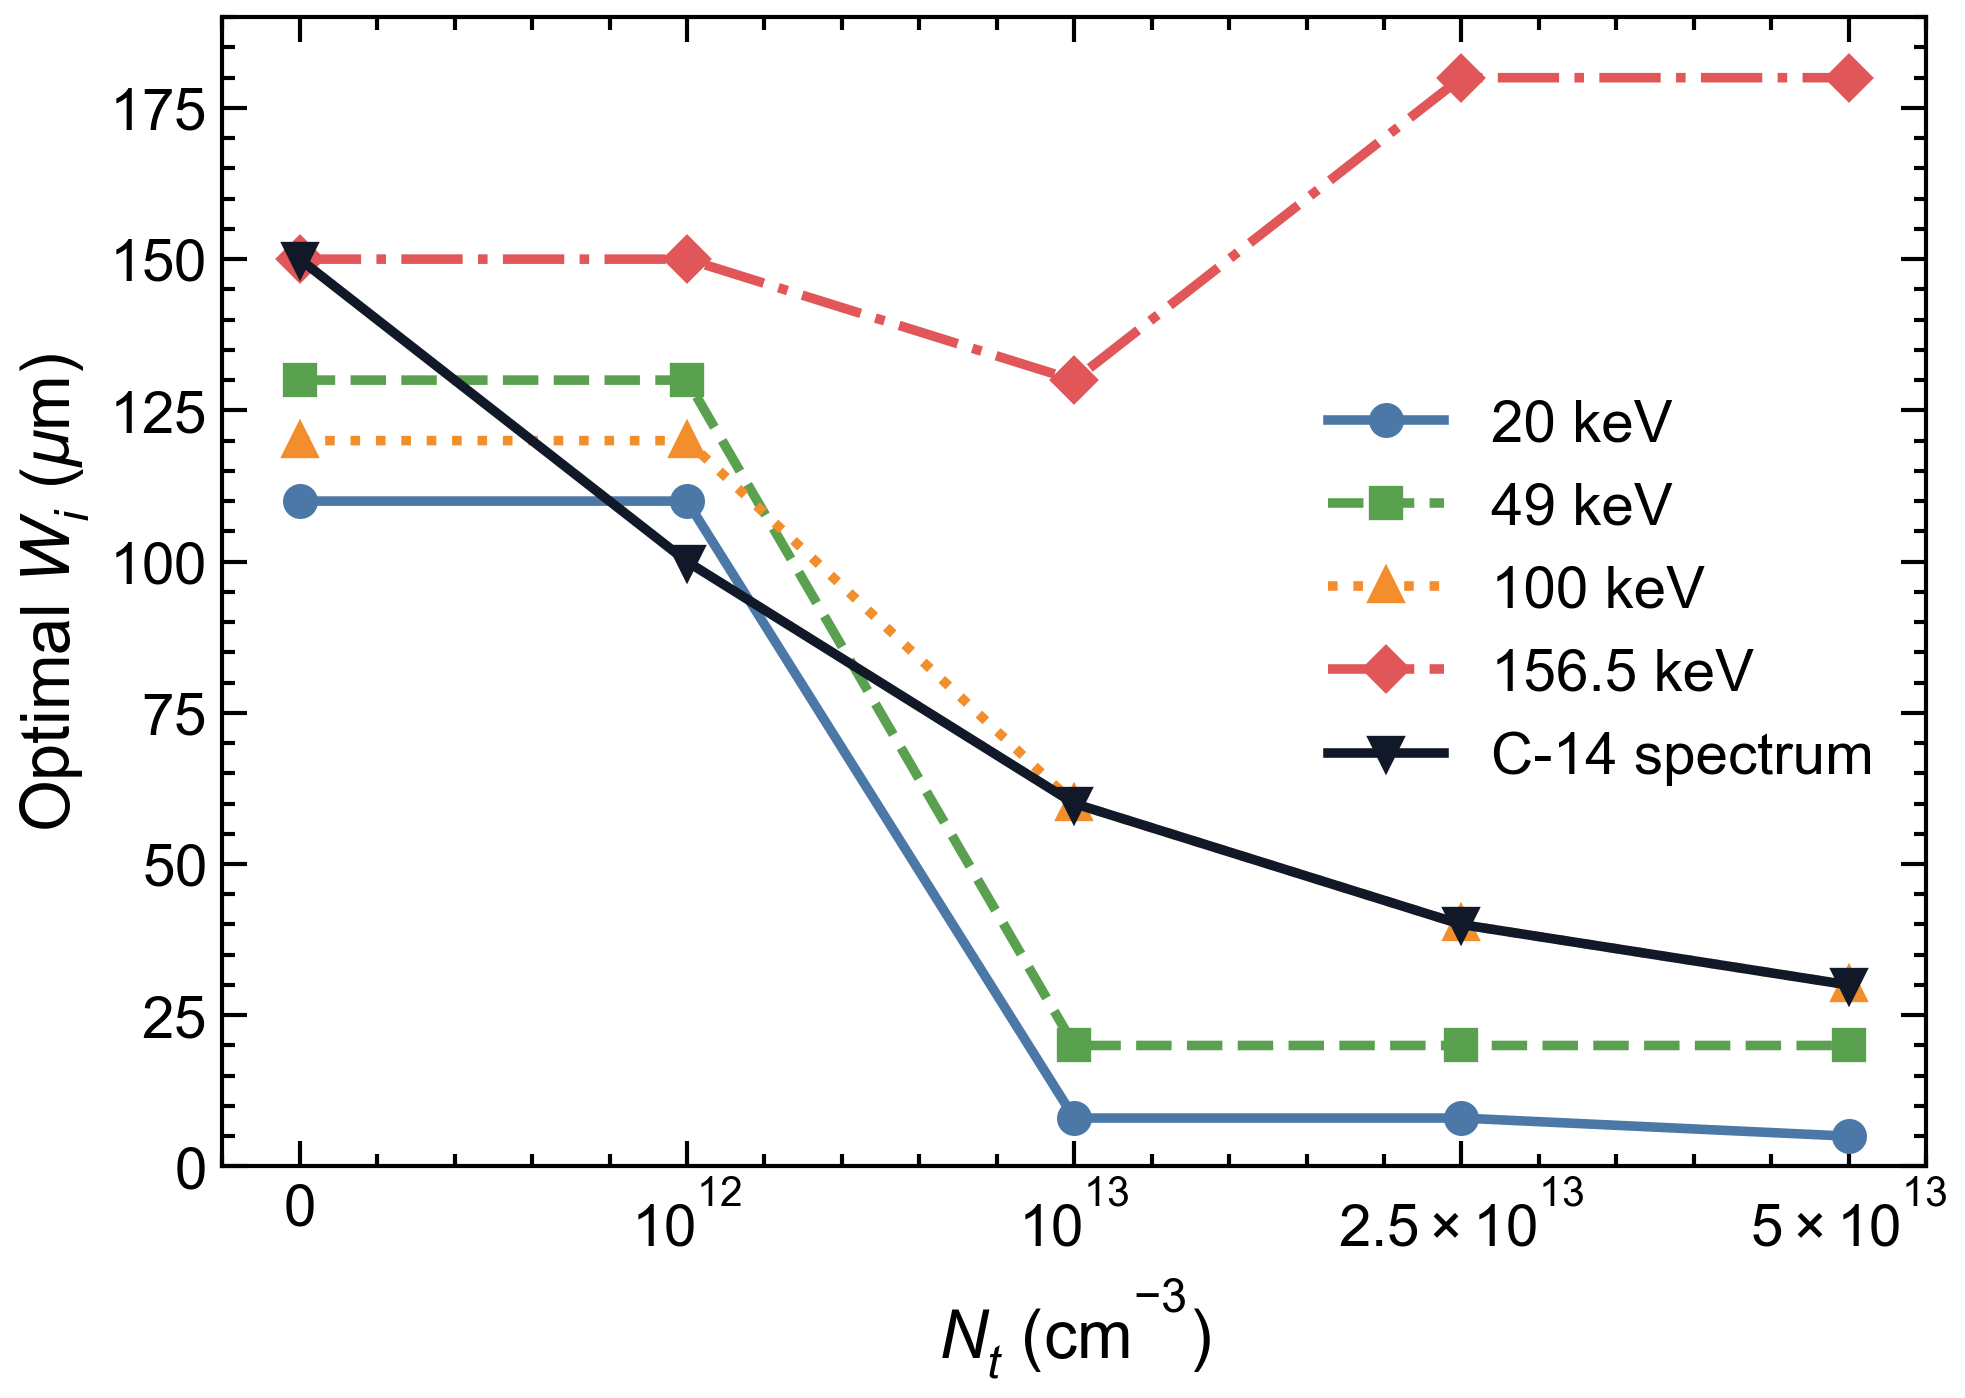
\includegraphics[keepaspectratio,alt={Fig.8 最优 i 区厚度随缺陷密度变化}]{figures/fig8_optimal_thickness_vs_Nt.png}}

\textbf{Fig.8.} 以最大 CCE 为准则得到的最优 i 区厚度随缺陷密度 \(N_t\)
的变化。五条曲线分别对应 20、49、100、156.5 keV 和 C-14 连续谱。

低缺陷密度下，多数源项的最优厚度位于 100-\(150\ \mu\mathrm{m}\)
的厚端区域，说明当材料质量足够高时，增加 i
区厚度可以更完整地覆盖高能电子的沉积尾部。随着 \(N_t\) 增加到
\(10^{13}\ \mathrm{cm^{-3}}\)，20 和 49 keV 的最优厚度分别回缩到 8 和
\(20\ \mu\mathrm{m}\)，100 keV 与 C-14 均回缩到
\(60\ \mu\mathrm{m}\)，而 156.5 keV 仍保持在
\(130\ \mu\mathrm{m}\)。进一步增大到
\(2.5\times10^{13}\ \mathrm{cm^{-3}}\) 后，100 keV 和 C-14
的最优厚度同步回缩到 \(40\ \mu\mathrm{m}\)；当
\(N_t=5\times10^{13}\ \mathrm{cm^{-3}}\) 时，20、49、100 keV 和 C-14
的最优厚度分别为 5、20、30 和 \(30\ \mu\mathrm{m}\)。156.5 keV
在高缺陷密度下仍偏向厚端，但其可达到的 CCE
已显著降低，说明单纯追求最高能端沉积覆盖会付出较大的俘获损失。

该结果表明，C-14 的最优厚度并不等同于 49 keV 平均能量或 156.5 keV
最高能量的最优厚度。真实连续谱同时包含浅层低能贡献和深层高能尾部，其设计点由谱形和材料缺陷共同决定。

五个源项的统计结果进一步显示，理想材料下最优厚度中位数为
\(130\ \mu\mathrm{m}\)，最优 CCE 中位数约为
97.8\%；\(N_t=10^{12}\ \mathrm{cm^{-3}}\) 时，中位最优厚度仍保持在
\(120\ \mu\mathrm{m}\)。当 \(N_t\) 增至 \(10^{13}\ \mathrm{cm^{-3}}\)
时，最优厚度中位数回缩至 \(60\ \mu\mathrm{m}\)，最优 CCE
中位数仍可保持在约 95.1\%。当 \(N_t=2.5\times10^{13}\) 和
\(5\times10^{13}\ \mathrm{cm^{-3}}\) 时，最优厚度中位数进一步回缩至 40
和 \(30\ \mu\mathrm{m}\)，最优 CCE 中位数分别下降至约 80.5\% 和
73.8\%。这说明厚度优化能够缓解材料缺陷带来的收集损失，但不能完全抵消高缺陷外延层造成的性能下降。

\textbf{Table 5. 五个源项的最优厚度统计。}

{\def\LTcaptype{none} % do not increment counter
\begin{longtable}[]{@{}
  >{\raggedleft\arraybackslash}p{(\linewidth - 8\tabcolsep) * \real{0.2000}}
  >{\raggedleft\arraybackslash}p{(\linewidth - 8\tabcolsep) * \real{0.2000}}
  >{\raggedleft\arraybackslash}p{(\linewidth - 8\tabcolsep) * \real{0.2000}}
  >{\raggedleft\arraybackslash}p{(\linewidth - 8\tabcolsep) * \real{0.2000}}
  >{\raggedleft\arraybackslash}p{(\linewidth - 8\tabcolsep) * \real{0.2000}}@{}}
\toprule\noalign{}
\begin{minipage}[b]{\linewidth}\raggedleft
\(N_t\) (cm\(^{-3}\))
\end{minipage} & \begin{minipage}[b]{\linewidth}\raggedleft
最优厚度中位数 (\(\mu\)m)
\end{minipage} & \begin{minipage}[b]{\linewidth}\raggedleft
最优厚度均值 (\(\mu\)m)
\end{minipage} & \begin{minipage}[b]{\linewidth}\raggedleft
相对 \(N_t=0\) 的中位回缩 (\(\mu\)m)
\end{minipage} & \begin{minipage}[b]{\linewidth}\raggedleft
最优 CCE 中位数 (\%)
\end{minipage} \\
\midrule\noalign{}
\endhead
\bottomrule\noalign{}
\endlastfoot
0 & 130 & 132 & 0 & 97.80 \\
\(10^{12}\) & 120 & 122 & 10 & 97.72 \\
\(10^{13}\) & 60 & 55.6 & 70 & 95.09 \\
\(2.5\times10^{13}\) & 40 & 57.6 & 90 & 80.54 \\
\(5\times10^{13}\) & 30 & 53.0 & 100 & 73.78 \\
\end{longtable}
}

\subsubsection{3.6
单能近似造成的设计偏差}\label{ux5355ux80fdux8fd1ux4f3cux9020ux6210ux7684ux8bbeux8ba1ux504fux5dee}

为了定量评估用单能电子代替 C-14 连续谱的设计误差，本文固定实际入射源项为
C-14，并比较不同设计源项在各 \(N_t\) 下给出的最优厚度用于 C-14
时可达到的 CCE。Fig.9 采用三维散点图表示该交叉评估结果：横轴为缺陷密度
\(N_t\)，纵轴为设计源项，竖轴和散点颜色均为用于 C-14 时得到的
CCE，颜色越深表示性能越高。

\pandocbounded{
\includegraphics[keepaspectratio,alt={Fig.9 单能近似设计偏差三维图}]{figures/fig9_design_bias_matrix.png}}

\textbf{Fig.9.} 不同单能源项设计用于 C-14 连续谱时的 CCE
三维散点图。每个点对应一个 \(N_t\)
与一个设计源项组合，点的高度和颜色表示该设计用于 C-14 时得到的 CCE。

在低缺陷密度下，不同设计源项用于 C-14 时的 CCE 都接近
97.7\%-97.8\%，说明厚端饱和区掩盖了单能源项之间的差异。随着缺陷密度升高，不同设计源项之间的
CCE 差异被显著放大。对于 \(N_t=10^{13}\ \mathrm{cm^{-3}}\)，20 keV
设计对应的 C-14 CCE 仅约 50.8\%，而 C-14 和 100 keV 设计可达到约
95.1\%；156.5 keV 设计约为 72.2\%。对于
\(N_t=2.5\times10^{13}\ \mathrm{cm^{-3}}\)，20 keV 和 156.5 keV 设计用于
C-14 时分别只有约 50.8\% 和 51.7\%，而 C-14 和 100 keV 设计可达到约
87.1\%。对于 \(N_t=5\times10^{13}\ \mathrm{cm^{-3}}\)，20 keV 与 156.5
keV 设计用于 C-14 时分别只有约 37.1\% 和 40.7\%，而 C-14 和 100 keV
设计仍可达到约
81.7\%。这些结果说明，高缺陷条件下的厚度优化不能简单依赖平均能量或端点能量单能近似。

这说明单能近似是否可接受并不是一个固定结论，而取决于外延层缺陷密度。当材料质量较高时，厚端饱和掩盖了不同源项之间的设计差异；当材料缺陷较高时，谱形差异和陷阱俘获共同放大厚度选择误差。因此，C-14
探测器的厚度优化应直接使用真实连续谱，而不应默认采用平均能量或最大能量单能近似。

\subsection{4. 讨论}\label{ux8ba8ux8bba}

\subsubsection{4.1 CCE
作为唯一优化目标的合理性}\label{cce-ux4f5cux4e3aux552fux4e00ux4f18ux5316ux76eeux6807ux7684ux5408ux7406ux6027}

本文以 CCE
作为唯一品质因子，是因为目标问题是厚度选择而不是读出电路时间响应优化。对于
C-14 探测，器件几何与材料缺陷首先决定的是有多少由 β
粒子产生的电子-空穴对能够被实际收集。缺陷俘获、深层复合和厚度不足造成的能量沉积截断最终都直接表现为
\(Q_{\mathrm{collected}}/Q_{\mathrm{generated}}\) 的下降。因此，CCE
是连接粒子输运、器件结构和材料质量的最直接指标。

瞬态电流波形仍然是 CCE
积分的中间量，但本文不再引入额外的时间类品质因子。这样可以避免多目标权重选择带来的方法学分散，使主线集中于``给定外延材料质量时如何选择
i 区厚度以最大化电荷收集''。

\subsubsection{4.2
材料质量驱动的设计建议}\label{ux6750ux6599ux8d28ux91cfux9a71ux52a8ux7684ux8bbeux8ba1ux5efaux8bae}

由 C-14
连续谱结果可得到材料质量驱动的设计速查表。该表不是将某一厚度作为普适最优值，而是说明当外延层可达到的缺陷密度不同时，应如何选择
i 区厚度来最大化 CCE。

\textbf{Table 6. C-14 探测应用的材料质量驱动设计建议。}

{\def\LTcaptype{none} % do not increment counter
\begin{longtable}[]{@{}
  >{\raggedright\arraybackslash}p{(\linewidth - 8\tabcolsep) * \real{0.1579}}
  >{\raggedleft\arraybackslash}p{(\linewidth - 8\tabcolsep) * \real{0.2105}}
  >{\raggedleft\arraybackslash}p{(\linewidth - 8\tabcolsep) * \real{0.2105}}
  >{\raggedleft\arraybackslash}p{(\linewidth - 8\tabcolsep) * \real{0.2105}}
  >{\raggedleft\arraybackslash}p{(\linewidth - 8\tabcolsep) * \real{0.2105}}@{}}
\toprule\noalign{}
\begin{minipage}[b]{\linewidth}\raggedright
材料质量等级
\end{minipage} & \begin{minipage}[b]{\linewidth}\raggedleft
\(N_t\) (cm\(^{-3}\))
\end{minipage} & \begin{minipage}[b]{\linewidth}\raggedleft
推荐 \(W_i\) (\(\mu\)m)
\end{minipage} & \begin{minipage}[b]{\linewidth}\raggedleft
偏压 (V)
\end{minipage} & \begin{minipage}[b]{\linewidth}\raggedleft
预期 CCE (\%)
\end{minipage} \\
\midrule\noalign{}
\endhead
\bottomrule\noalign{}
\endlastfoot
理想参考材料 & 0 & 150 & 117 & 97.80 \\
低缺陷外延情形 & \(10^{12}\) & 100 & 52 & 97.72 \\
缺陷较丰富外延情形 & \(10^{13}\) & 60 & 19 & 95.09 \\
中高缺陷等效情形 & \(2.5\times10^{13}\) & 40 & 8 & 87.14 \\
严重缺陷上限情形 & \(5\times10^{13}\) & 30 & 5 & 81.72 \\
\end{longtable}
}

该表体现了本文的核心工程结论：高质量材料可以使用较厚 i 区以覆盖 C-14
高能尾部；缺陷密度较高时，继续增加厚度会显著放大俘获损失，推荐厚度应向薄端回缩。表中的材料质量描述是等效
TCAD
设计情形，不应理解为对商业外延片的严格产业分级。实际器件设计中，\(N_t\)
可由 DLTS、少子寿命或等效 TCAD
校准获得，随后从该设计图中读取推荐厚度范围。

需要注意的是，本文扫描到的最厚结构用于探索物理趋势，并不意味着所有厚度都具有相同工程可用性。根据一维耗尽估算，\(W_i=180\ \mu\mathrm{m}\)
时所需全耗尽偏压显著高于薄器件，在便携式或低功耗 C-14
系统中可能带来高压供电、漏电流和封装可靠性限制。因此，最终工程设计还应叠加允许偏压、暗电流和系统功耗约束。对于本文
C-14 主线结果，高缺陷材料的推荐厚度本身已经回缩到 30-60
\(\mu\)m，对应偏压处于更易实现的范围；理想或低缺陷材料中的厚端方案则应结合具体高压读出条件进一步筛选。

\subsubsection{4.3
与已有文献的间接验证}\label{ux4e0eux5df2ux6709ux6587ux732eux7684ux95f4ux63a5ux9a8cux8bc1}

本文结论可与已有 4H-SiC 探测器和外延层质量研究进行间接对照。Moscatelli
等对 SiC \(p^+/n\) 结探测器的 CCE 测量与仿真表明，合适的 TCAD
模型能够再现实验电荷收集趋势 {[}6{]}。He 等采用 SRIM/TCAD 分析 SiC α
粒子探测器瞬态响应，说明粒子输运结果向 TCAD 载流子产生项映射是研究 SiC
探测器瞬态响应的可行路线 {[}7{]}；本文与其区别在于源项为 C-14 连续 β
谱，并进一步把厚度和外延陷阱密度作为二维设计变量。Kleppinger 等对
50、150 和 \(250\ \mu\mathrm{m}\) 4H-SiC
外延层的研究显示，厚外延层的缺陷和材料质量会显著影响探测器性能；这与本文关于``厚器件对缺陷更敏感''的趋势一致。Kimoto
与 Capan 等对 SiC 外延生长和电活性缺陷的综述也支持本文将 Z1/2
作为外延层主要电活性缺陷纳入模型 {[}15{]}, {[}18{]}。

此外，4H-SiC betavoltaic
优化工作通常也面对类似的厚度-材料质量权衡：较厚吸收层可提高 β
能量吸收，但会引入更强的复合损失。Kim 等对 4H-SiC betavoltaic cell
的结构和陷阱效应研究表明，陷阱密度升高会降低输出性能，并使结构优化结果依赖材料质量
{[}19{]}。本文虽然研究对象是探测器而非电池，但 CCE-厚度-\(N_t\)
设计图与这类``吸收厚度增加''和``复合/俘获损失增加''的竞争问题具有共同物理基础。

\subsubsection{4.4 模型局限}\label{ux6a21ux578bux5c40ux9650}

本文仍存在若干局限。第一，载流子输运采用漂移-扩散近似，尚未包含全 Monte
Carlo
载流子输运。第二，表面复合、边缘场和封装窗口材料被简化处理，这可能影响
20 keV 等低能电子的近表面响应。第三，缺陷模型仅包含 Z1/2 和 EH6/7
两类主导中心，未纳入所有可能的次要深能级，也未扫描两类中心的相对浓度和俘获截面。第四，本文只讨论室温条件，温度对迁移率、寿命和陷阱俘获动力学的影响需要后续研究。第五，瞬态积分窗口、时间步长和初始条件仍需结合实验响应进一步校准。

后续工作应优先围绕三类验证展开：首先，用 NIST ESTAR 或已报道 SiC PIN
探测器 CCE 数据对 Geant4 能量沉积和 TCAD
收集电荷进行量化校准；其次，扫描
\(N_{\mathrm{Z1/2}}/N_{\mathrm{EH6/7}}\)、\(\sigma_e\) 和
\(\sigma_h\)，给出最优厚度对缺陷参数不确定性的敏感性范围；最后，引入 p+
死区、表面复合和电子学噪声模型，评估低能 β
响应和脉冲高度分布。完成这些验证后，本文的参数化设计图才能进一步转化为面向具体器件工艺的设计准则。

\subsection{5. 结论}\label{ux7ed3ux8bba}

本文建立了面向 C-14 连续 β 谱的 Geant4-Sentaurus
耦合仿真框架，并将其用于 4H-SiC PIN 探测器 i
区厚度和外延缺陷密度的二维设计优化。

第一，Geant4 结果表明，C-14 连续谱在 SiC
中形成的能量沉积分布同时包含浅层低能贡献和高能深层尾部，不能由 49 keV
平均能量或 156.5 keV 最大能量的单能源项完整替代。

第二，以 CCE 为唯一优化目标时，理想材料中 CCE 随 i
区厚度增加而趋于饱和；引入 Z1/2 和 EH6/7
深能级缺陷后，厚端载流子俘获损失增强，CCE 转变为非单调函数，最优 i
区厚度自然出现。

第三，C-14 连续谱的最优厚度随材料缺陷密度系统性变化。完整数据表明，C-14
最优厚度从 \(N_t=0\) 时的 \(150\ \mu\mathrm{m}\) 和
\(N_t=10^{12}\ \mathrm{cm^{-3}}\) 时的 \(100\ \mu\mathrm{m}\)，回缩到
\(N_t=10^{13}\)、\(2.5\times10^{13}\) 和
\(5\times10^{13}\ \mathrm{cm^{-3}}\) 下的 60、40 和
\(30\ \mu\mathrm{m}\)。对应最优 CCE 分别约为
97.8\%、97.7\%、95.1\%、87.1\% 和 81.7\%。

第四，单能近似造成的厚度设计误差会随缺陷密度增大而放大。在低缺陷材料中，不同源项的最优厚度均处于厚端饱和区，用于
C-14 的交叉 CCE 损失通常低于 0.1 个百分点；在高缺陷材料中，使用 20 keV
或 156.5 keV 代替 C-14 进行设计可造成 35-45 个百分点量级的 CCE
损失。因此，C-14 探测器的厚度优化应直接使用真实连续谱。

综上，本文给出了一种基于外延材料质量等级的 4H-SiC PIN C-14
探测器厚度选择方法。该方法可进一步推广到 Ni-63、H-3 等其他低能 β
源，以及 betavoltaic 电池中吸收层厚度与材料质量的协同优化。

\subsection{参考文献}\label{ux53c2ux8003ux6587ux732e}

{[}1{]} T. Kimoto and J. A. Cooper, \emph{Fundamentals of Silicon
Carbide Technology}, Wiley, 2014.

{[}2{]} F. Nava, G. Bertuccio, A. Cavallini, and E. Vittone, ``Silicon
carbide and its use as a radiation detector material,''
\emph{Measurement Science and Technology}, vol.~19, 102001, 2008.

{[}3{]} M. De Napoli, ``SiC detectors: A review on the use of silicon
carbide as radiation detection material,'' \emph{Frontiers in Physics},
vol.~10, 898833, 2022.

{[}4{]} M. V. Dolgopolov and A. S. Chipura, ``Heterojunction betavoltaic
Si14C-Si energy converter,'' \emph{Journal of Power Sources}, vol.~610,
234896, 2024.

{[}5{]} A. V. Gurskaya, A. A. Ivanov, A. V. Kiselev, and A. A.
Solodovnikov, ``SiC/Si-based converter of C-14 beta decay energy,''
\emph{Physics of Particles and Nuclei}, vol.~48, pp.~941-944, 2017.

{[}6{]} F. Moscatelli et al., ``Measurements and simulations of charge
collection efficiency of p+/n junction SiC detectors,'' \emph{Nuclear
Instruments and Methods in Physics Research A}, vol.~546, pp.~218-221,
2005.

{[}7{]} J. He et al., ``Transient behaviour analysis in silicon carbide
alpha particle detector using TCAD and SRIM simulation,'' \emph{Physica
Scripta}, vol.~99, 075943, 2024.

{[}8{]} A. Gsponer et al., ``Extraction of electron and hole drift
velocities in thin 4H-SiC PIN detectors using high-frequency readout
electronics,'' \emph{Sensors}, vol.~25, 7196, 2025.

{[}9{]} S. Agostinelli et al., ``Geant4: A simulation toolkit,''
\emph{Nuclear Instruments and Methods in Physics Research A}, 2003.

{[}10{]} J. Allison et al., ``Recent developments in Geant4,''
\emph{Nuclear Instruments and Methods in Physics Research A}, 2016.

{[}11{]} A. Gsponer et al., ``Measurement of the electron-hole pair
creation energy in a 4H-SiC p-n diode,'' \emph{Nuclear Instruments and
Methods in Physics Research A}, vol.~1064, 169412, 2024.

{[}12{]} Synopsys, \emph{Sentaurus Device User Guide}, Synopsys Inc.

{[}13{]} NIST, ``ESTAR: Stopping-power and range tables for electrons,''
National Institute of Standards and Technology.

{[}14{]} M. Batic et al., ``Validation of Geant4 simulation of electron
energy deposition,'' \emph{IEEE Transactions on Nuclear Science},
vol.~60, pp.~2934-2941, 2013.

{[}15{]} T. Kimoto, ``Bulk and epitaxial growth of silicon carbide,''
\emph{Progress in Crystal Growth and Characterization of Materials},
2016.

{[}16{]} K. Kleppinger et al., ``Carrier trapping in 4H-SiC epitaxial
layers with different thicknesses,'' \emph{Journal of Crystal Growth},
2022.

{[}17{]} P. Gaggl et al., ``TCAD modeling of radiation-induced defects
in 4H-SiC diodes,'' \emph{Nuclear Instruments and Methods in Physics
Research A}, vol.~1070, 170015, 2025.

{[}18{]} I. Capan, ``Electrically active defects in 3C, 4H, and 6H
silicon carbide polytypes: A review,'' \emph{Crystals}, vol.~15, 255,
2025.

{[}19{]} K. M. Kim, I. M. Kang, J. H. Seo, Y. J. Yoon, and K. Kim,
``Structural optimization and trap effects on the output performance of
4H-SiC betavoltaic cell,'' \emph{Nanomaterials}, vol.~15, 1625, 2025.

\end{document}
